\documentclass{beamer}

%% \documentclass[handout]{beamer}
%% % use this with the [handout] option to create handouts for the audience
%% \usepackage{pgfpages}
%% \pgfpagesuselayout{2 on 1}[a4paper,border shrink=5mm]

\mode<presentation>
{
  \usetheme{Diku}
% set this to your preferences:
  \setbeamercovered{invisible}
%  \setbeamercovered{transparent}
}

\usepackage{graphicx}
\usepackage{epic}

\usepackage{amsmath}
\usepackage{amssymb}
\usepackage{amsthm}

\newcommand{\basetop}[1]{\vtop{\vskip-1ex\hbox{#1}}}
\newcommand{\source}[1]{\let\thefootnote\relax\footnotetext{\scriptsize\textcolor{kugray1}{Source: #1}}}

% for coloured code citation in text:
\usepackage{fancyvrb}

%%%%%%%%%%%%%%%%%%%%%%%%%%%%%%%%%
%%%%%    code sections   %%%%%%%%
%%%%%%%%%%%%%%%%%%%%%%%%%%%%%%%%%

% code highlighting commands in own block
\DefineVerbatimEnvironment{code}{Verbatim}{fontsize=\scriptsize}
\DefineVerbatimEnvironment{icode}{Verbatim}{fontsize=\scriptsize}

% Fancy code with color commands:
\DefineVerbatimEnvironment{colorcode}%
        {Verbatim}{fontsize=\scriptsize,commandchars=\\\{\}}

%%%%%%%%%%%%%%%%%%%%%%%%%%%%%%%%%%
%%%%%    some coloring    %%%%%%%%

% use "DIKU green" from our color theme for \emph
\renewcommand{\emph}[1]{\textcolor{structure}{#1}}
% use some not-too-bright red for an \emp command
\definecolor{DikuRed}{RGB}{130,50,32}
\newcommand{\emp}[1]{\textcolor{DikuRed}{ #1}}
\definecolor{CosGreen}{RGB}{10,100,70}
\newcommand{\emphh}[1]{\textcolor{CosGreen}{ #1}}
\definecolor{CosBlue}{RGB}{55,111,122}
\newcommand{\emphb}[1]{\textcolor{CosBlue}{ #1}}
\definecolor{CosRed}{RGB}{253,1,1}
\newcommand{\empr}[1]{\textcolor{CosRed}{ #1}}

\newcommand{\mymath}[1]{$ #1 $}
\newcommand{\myindx}[1]{_{#1}}
\newcommand{\myindu}[1]{^{#1}}

\newtheorem{mydef}{Definition}
\newtheorem{mytheo}{Theorem}
\newtheorem{mylemma}{Lemma}


%%%%%%%%%%%%%%%%%%%%

\title[Parallelism History]{A Story of Parallelism: from\\ Imperative and Functional Languages}

\author[C.Oancea]{Cosmin E. Oancea \texttt{cosmin.oancea@diku.dk}}
\institute{HIPERFIT, Department of Computer Science\\University of Copenhagen}

\date[04.02.13 - Invited Lecture]{04.02.13 -- Invited Lecture for the Advanced Compiler Course}

\begin{document}

\titleslide

%%%%%%%% real content starts here %%%%%%%%%%

\begin{frame}
  \frametitle{Motivation}
  

Parallel hardware is here to stay, e.g., general-purpose graphic processing units ({\sc gpgpu}).

\bigskip

Powerful graphical cards are fundamental to gaming ...

\center 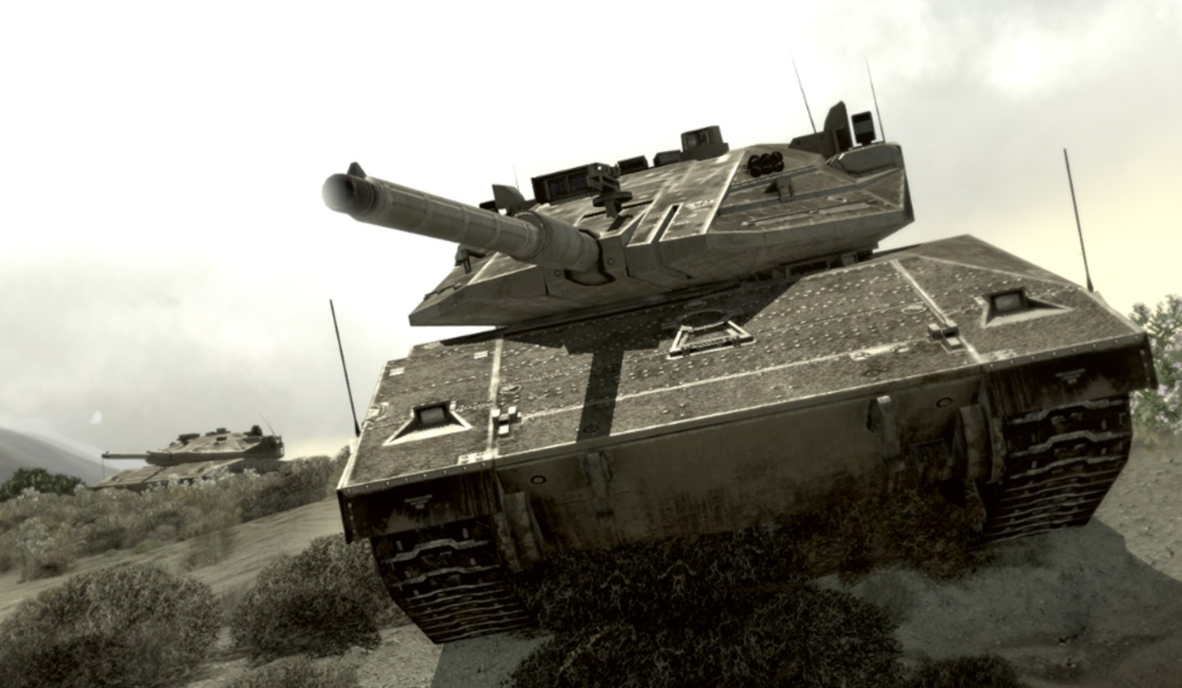
\includegraphics[height=30ex]{ParTeaserFigs/tank}  %\pause %\bigskip

\end{frame}


\begin{frame}
  \frametitle{Motivation}
  %\centering
\bigskip
... and ({\sc gpgpu}s) have also been used in other areas of less impact: \bigskip 

weather prediction, 
$\mbox{ }\mbox{ }\mbox{ }\mbox{ }\mbox{ }\mbox{ }\mbox{ }\mbox{ }\mbox{ }\mbox{ }\mbox{ }\mbox{ }\mbox{ }\mbox{ }\mbox{ }\mbox{ }$ 
$\mbox{ }\mbox{ }\mbox{ }\mbox{ }\mbox{ }\mbox{ }\mbox{ }$
bioinformatics,

\begin{center} 
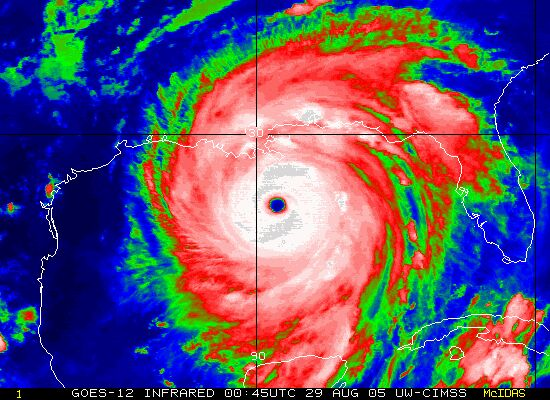
\includegraphics[height=15ex]{ParTeaserFigs/meteo}  
$\mbox{ }\mbox{ }\mbox{ }\mbox{ }\mbox{ }\mbox{ }\mbox{ }\mbox{ }\mbox{ }\mbox{ }\mbox{ }\mbox{ }\mbox{ }\mbox{ }\mbox{ }\mbox{ }$ 
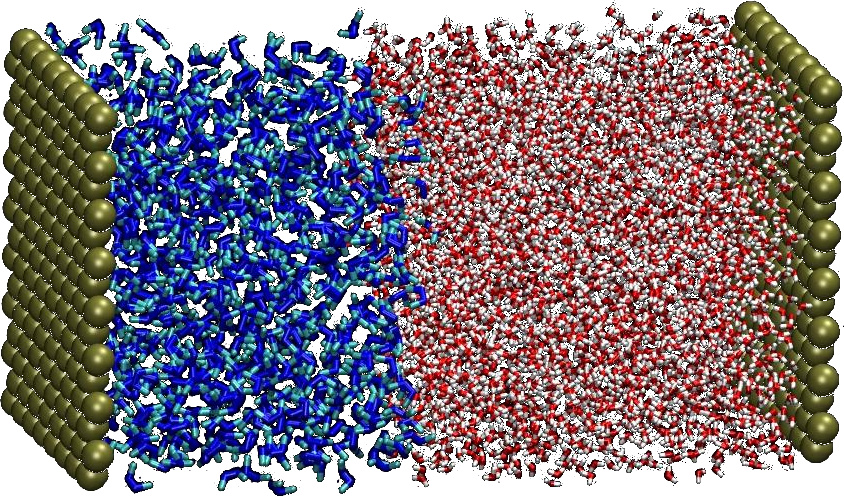
\includegraphics[height=15ex]{ParTeaserFigs/molecular_sim.jpg}  
\end{center} 
\smallskip

fluid-dynamic simulations,
$\mbox{ }\mbox{ }\mbox{ }\mbox{ }\mbox{ }\mbox{ }\mbox{ }\mbox{ }\mbox{ }\mbox{ }\mbox{ }\mbox{ }\mbox{ }\mbox{ }\mbox{ }\mbox{ }$ 
finance

\begin{center} 
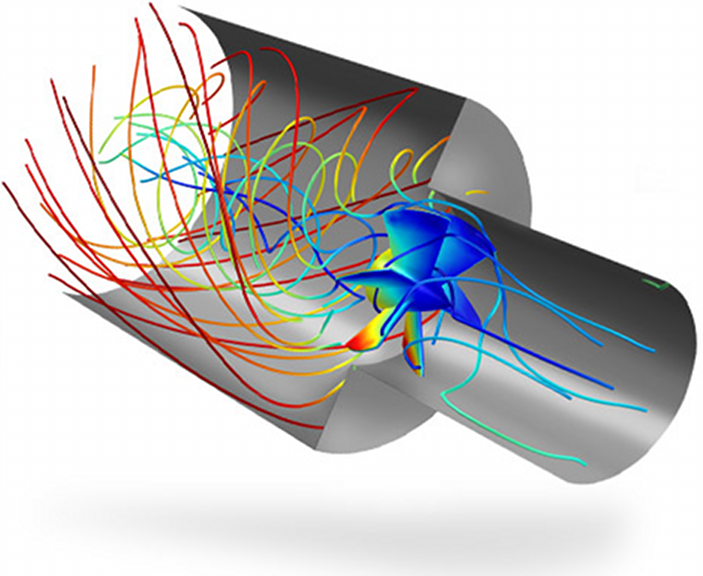
\includegraphics[height=15ex]{ParTeaserFigs/fluid_dyn_sim.png}  
$\mbox{ }\mbox{ }\mbox{ }\mbox{ }\mbox{ }\mbox{ }\mbox{ }\mbox{ }\mbox{ }\mbox{ }\mbox{ }\mbox{ }\mbox{ }\mbox{ }\mbox{ }\mbox{ }$ 
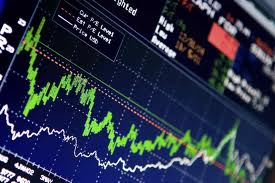
\includegraphics[height=15ex]{ParTeaserFigs/finance.jpeg} 
\end{center}
\end{frame}


\begin{frame}[fragile]
	\tableofcontents
\end{frame}

\section{Brief History of Hardware and High-Level Comparison}


\begin{frame}
  \frametitle{Brief Hardware History} 
  \centering
\begin{itemize}
    \item How did general-purpose graphics-processing units (\emph{{\sc gpgpu}}) come to being?\bigskip 
    
    \item In the beginning was the \emph{Single-CPU},\smallskip \\ 
            and the \emph{single-CPU} was sequentially-programmable,\smallskip \\ 
            and sequential code was programming.\bigskip

    \item Then the frequency of the single-CPU could not be further increased 
            and \emph{Multi-cores/processors} became mainstream. \bigskip

    \item And ``Hardware Engineers'' worked hard to support the illusion that 
            random-access to memory has uniform cost: \\ \smallskip
        \begin{itemize}
            \item   thrown many transistors to memory-hierarchy coherency and such\\ \smallskip
            \item   ... and ultimately (arguably) they have failed (to scale up)!
        \end{itemize} \bigskip
\bigskip

    \item But, but, but ... is the sequentially-written code going to benefit?
\end{itemize}
\end{frame}



\begin{frame}[fragile,t]
  \frametitle{Multicore Issues} 

What is the main cost of manual parallelization?\\
\begin{itemize}
    \item learning various tools, e.g., OpenMP, MPI, Intel-Basic Blocks?
    \item rewriting the code using those tools?
    \item ensuring that the parallel and sequential programs are equivalent?
\end{itemize}

\pause
\smallskip

Last one! Even reasoning about multicore hardware is nontrivial and error-prone.
Furthermore, \emp{hardware instructions, such as memory fences and 
compare-and-swap (CAS) do not seem to scale.}

%i.e., many bugs and unspecified behaviors in hardware doc, e.g., IA32.

\smallskip


\begin{block}{Memory Sequential Consistency (Memory Reordering)}
\begin{colorcode}[fontsize=\small]
         //Initially x = 0; y = 0;
//CORE 0                           //CORE 1
x = 1;                             y = 1;
//mfence;                          //mfence;
write(y);                          write(x);
\end{colorcode}
\end{block} 

%.. = y;                            .. = x;


\pause

No possible interleaving of instructions can result in both {\tt x} and {\tt y} 
being $0$ at the end. And still it happens. Fixed with {\tt mfences}.


\end{frame}


\begin{frame}
  \frametitle{Brief Hardware History (Continuation)} % of CPU, Multicores, GPGPU
  \centering
 \begin{itemize}
    \item Then ``Hardware Engineers'' fixed \emph{scalability} with \emph{{\sc gpgpu}} but took away \emp{programming convenience}:  \smallskip
        \begin{itemize}
            \item single-instruction multiple-data ({\sc simd}): 
                \begin{itemize}
                    \item cannot make an omelet with one core and a steak with the next,
                    \item but you can make first an omelet, then a steak, both very fast. 
                \end{itemize}\smallskip
            \item non-uniform, explicitly programmable memory hierarchy.\smallskip
            \item no dynamic allocation, no stack.\smallskip
            \item can only synchronize ``locally'' via barriers,
            \item \# cores $\sim$ thousands $\Rightarrow$ not enough to $||$ only the outermost loop!
        \end{itemize}
\end{itemize}

\begin{center} 
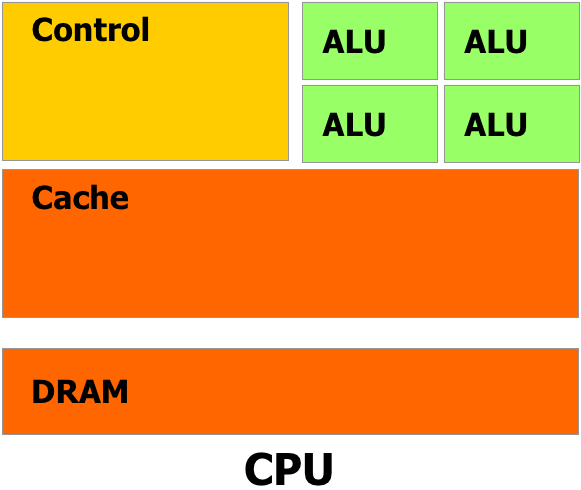
\includegraphics[height=20ex]{ParTeaserFigs/MulticoreArch.png}  
$\mbox{ }\mbox{ }\mbox{ }\mbox{ }\mbox{ }\mbox{ }\mbox{ }\mbox{ }\mbox{ }\mbox{ }\mbox{ }\mbox{ }\mbox{ }\mbox{ }\mbox{ }\mbox{ }$ 
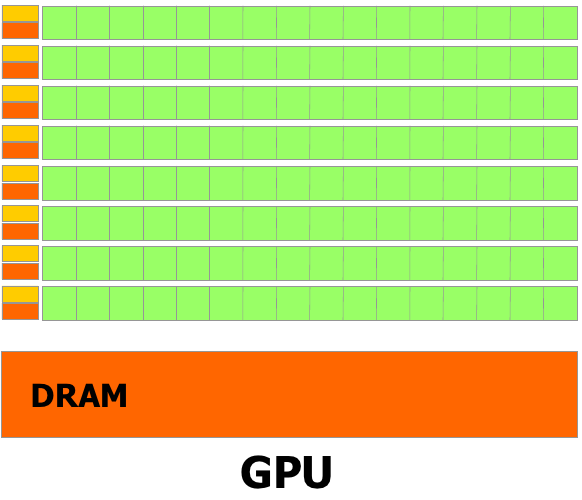
\includegraphics[height=20ex]{ParTeaserFigs/GPGPUarch.png}  
\end{center} 
\end{frame}


\begin{frame}
  \frametitle{Theoretical Hardware Comparison: CPU vs GPGPU} % of CPU, Multicores, GPGPU

\smallskip

{\sc gpgpu} shows superior peak bandwidth and compute power vs. {\sc cpu}.

\smallskip

\begin{center} 
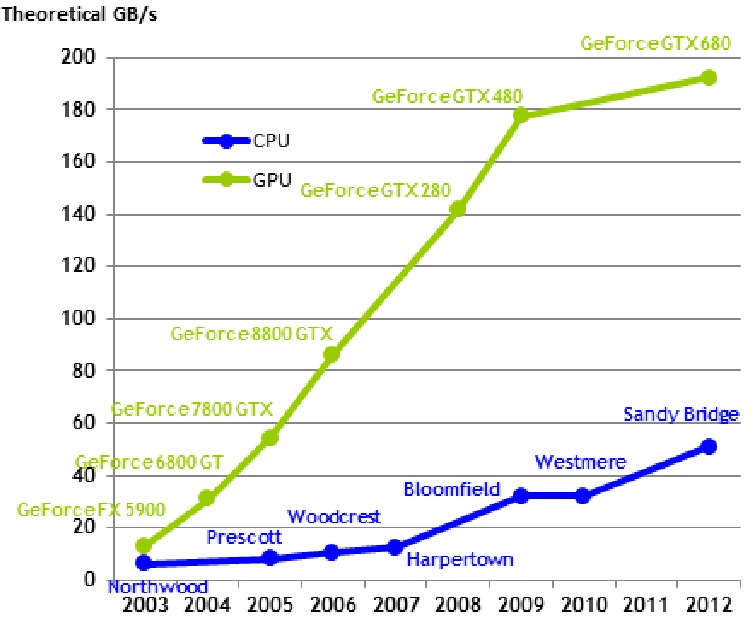
\includegraphics[height=27ex]{ParTeaserFigs/Bandwidth.png}  
%$\mbox{ }$ 
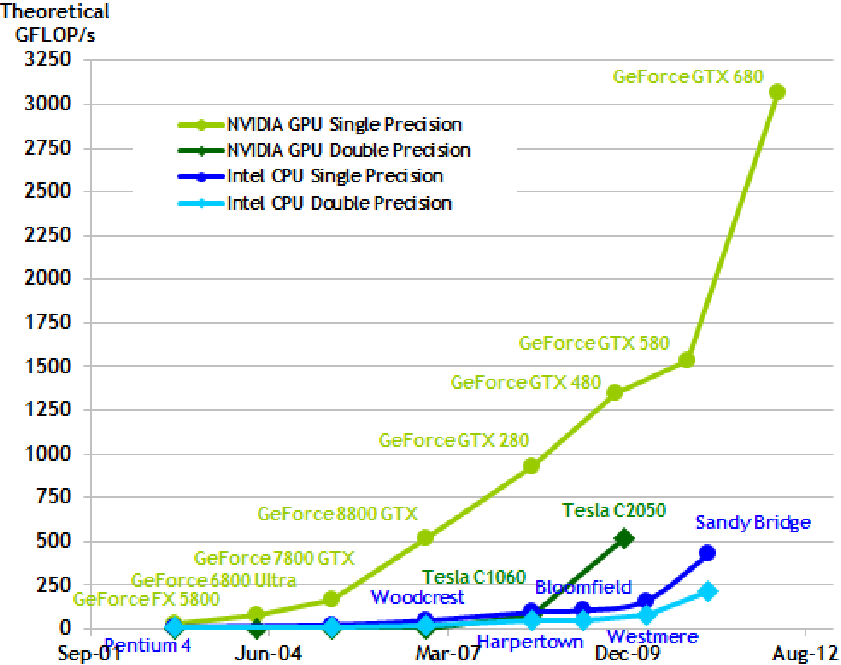
\includegraphics[height=27ex]{ParTeaserFigs/GFlops.png}
\end{center} 

\smallskip

\emp{However, peak bandwidth requires coalesced accesses}, i.e., if the cores executing
the (same) instruction access consecutive memory locations then the data is brought in
via {\em a single} memory transfer.

\end{frame}

\begin{frame}[fragile,t]
  \frametitle{Example of GPU programming} % of CPU, Multicores, GPGPU

\smallskip
\emp{\textsc{gpGPU} no dynamic allocation: what to do with local array variables?}

\pause
\smallskip

\begin{block}{ Loop Fusion $\mbox{~~~~~~~~~~~~~~~~~~~~~~~~~~~~~~~~~}$ Loop Distribution }
\begin{columns}
\column{0.45\textwidth}\vspace{-2ex}
\begin{colorcode}[fontsize=\scriptsize]
DO i = 1, N   \emphh{// Parallel}
  FLOAT A[M];  \emp{// local}
  DO j = 1, M  
    A[j] = ... f(i) ...
  ENDDO

  DO j = 1, M  
    A[j] = ... g(A[j]) ...
  ENDDO

  FLOAT sum = 0.0
  DO j = 1, M
    sum += A[j];
  ENDDO
  X[i] = sum;
ENDDO
\end{colorcode} 
\column{0.45\textwidth}\vspace{-2ex}
\begin{colorcode}[fontsize=\scriptsize]
FLOAT A[N,M];  \emp{// global}
DO i = 1, N   \emphh{// Parallel}
  DO j = 1, M  
    A[i,j] = ... f(i) ...
  ENDDO
ENDDO
DO i = 1, N   \emphh{// Parallel}
  DO j = 1, M  
    A[i,j] = ... g(A[i,j]) ...
  ENDDO
  real sum = 0.0
  DO j = 1, M
    sum += A[i,j];
  ENDDO
  X[i] = sum;
ENDDO
\end{colorcode}
\end{columns}
\end{block}

\end{frame}


%\visible<2-4>{
%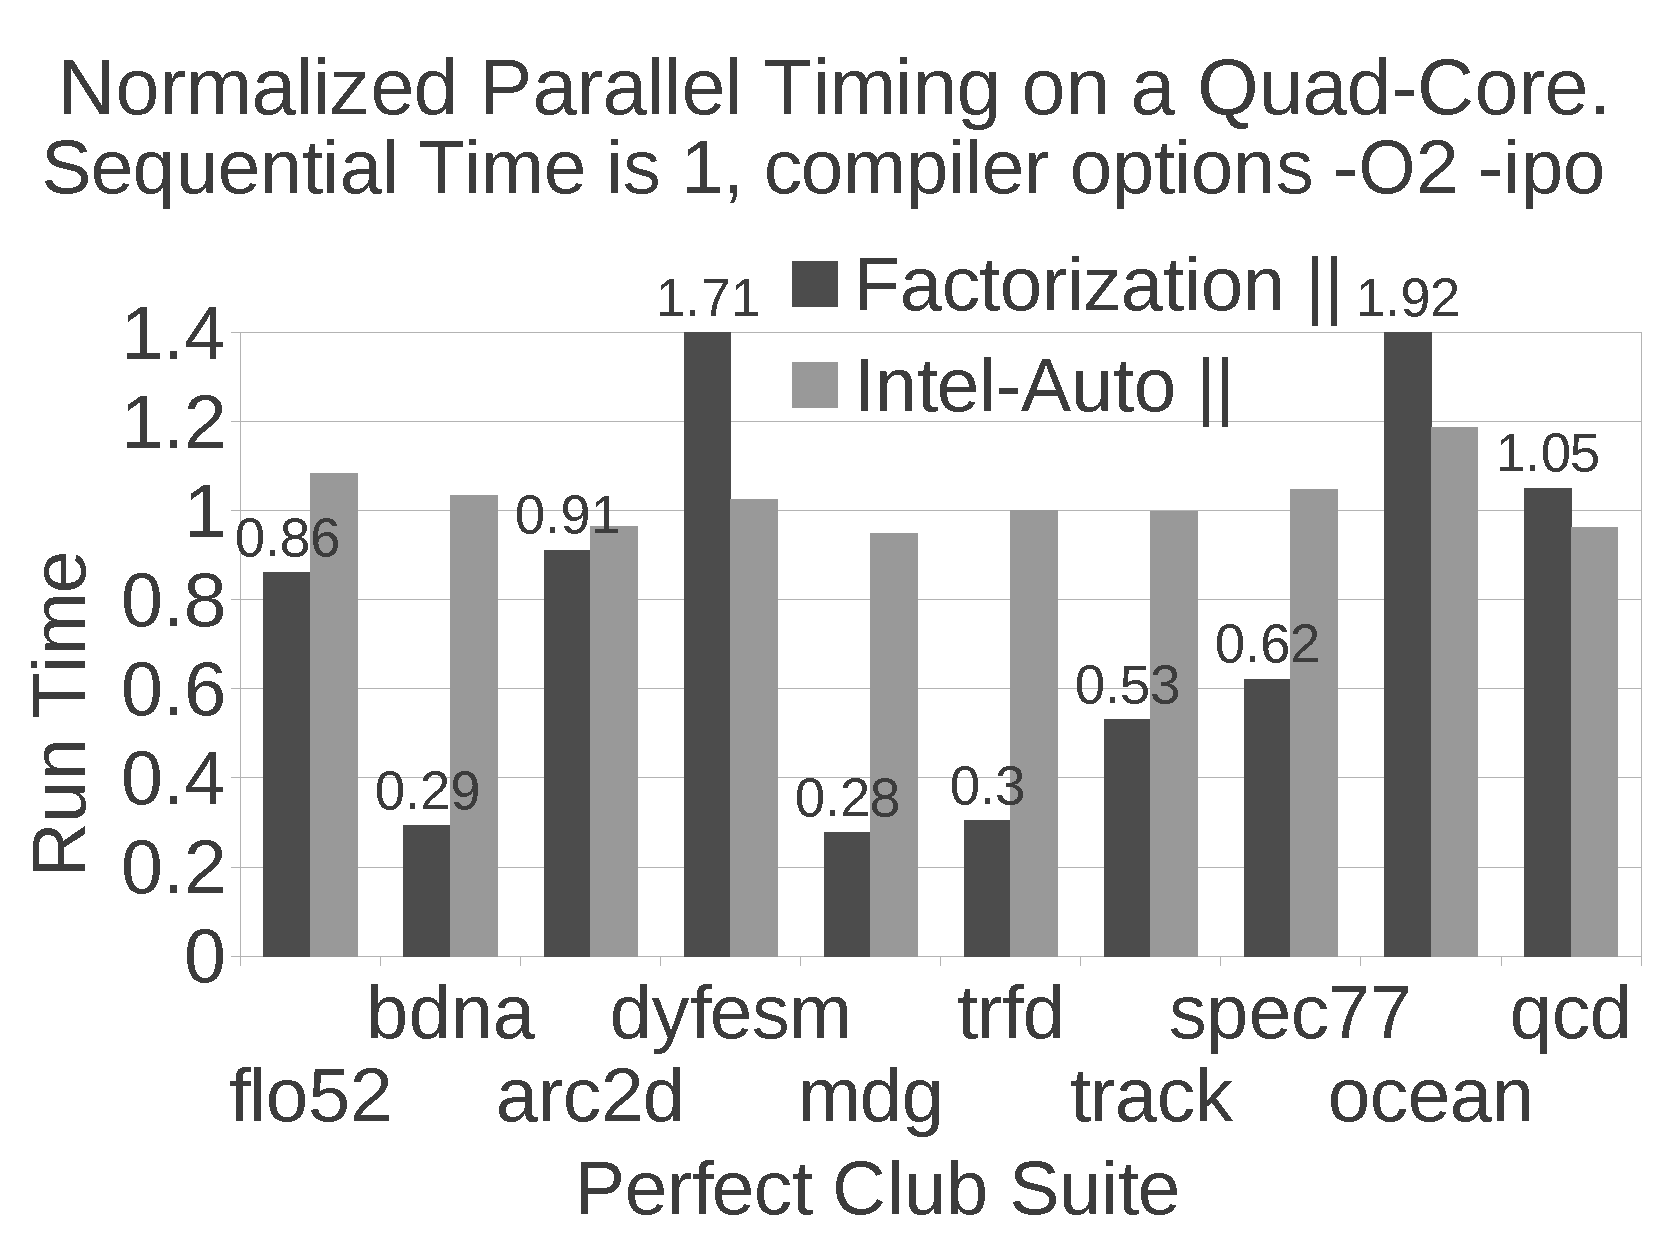
\includegraphics[scale=0.215]{ParTeaserFigs/PerfectResO2.pdf} } 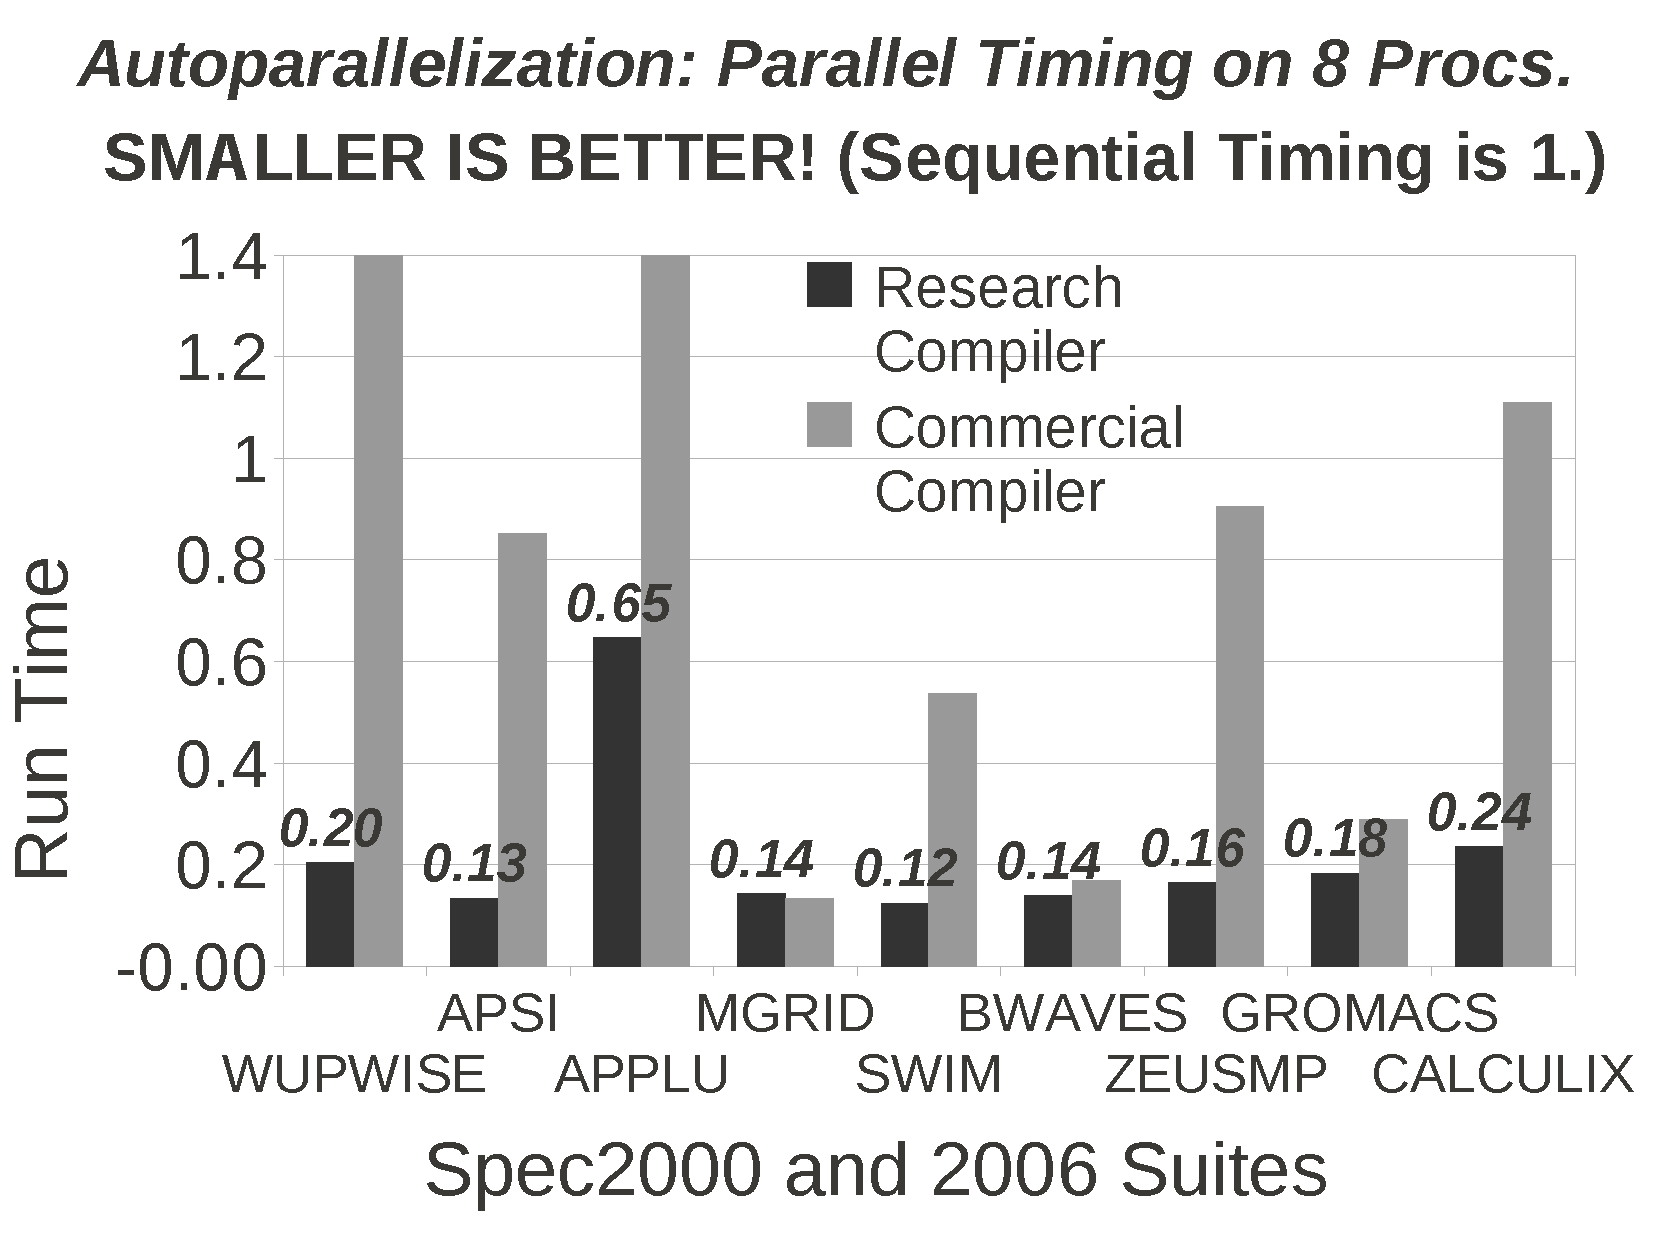
\includegraphics[scale=0.215]{ParTeaserFigs/Spec2006Res}
%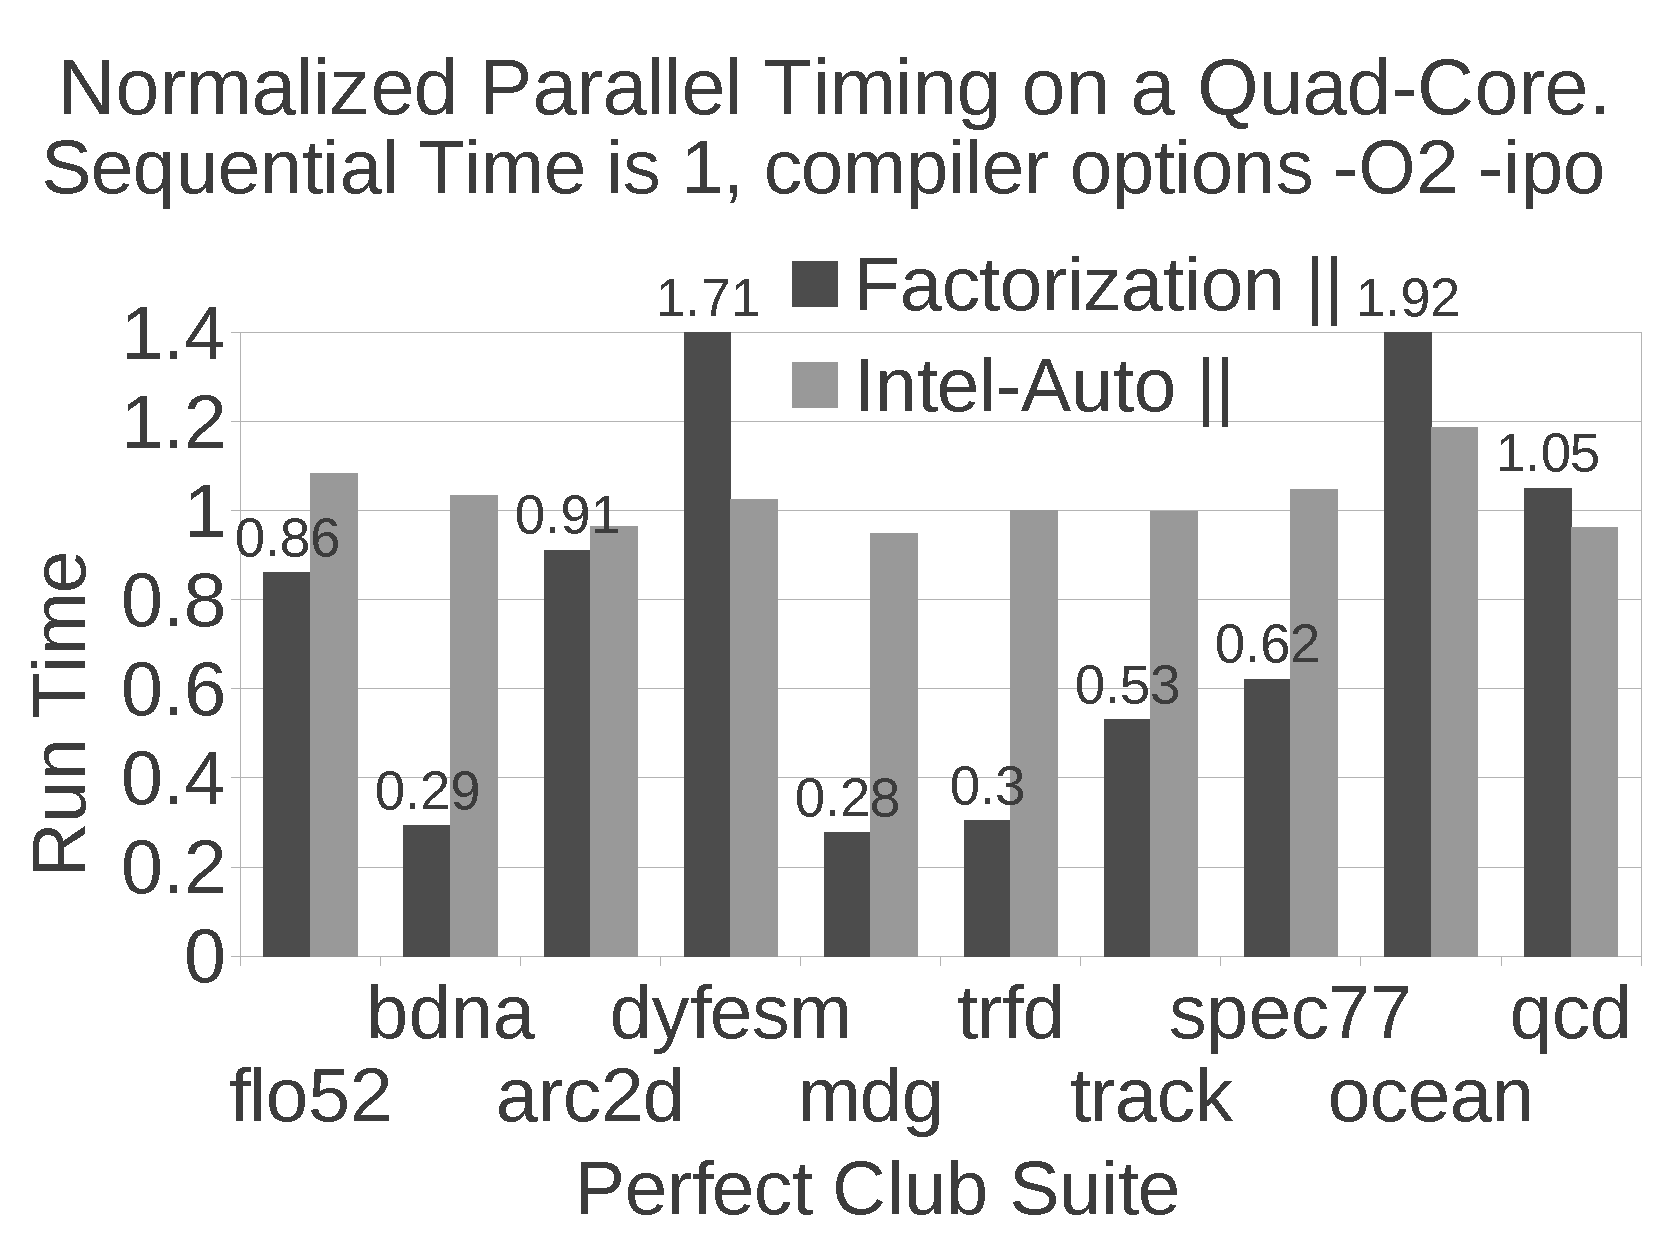
\includegraphics[scale=0.215]{ParTeaserFigs/PerfectResO2.pdf}  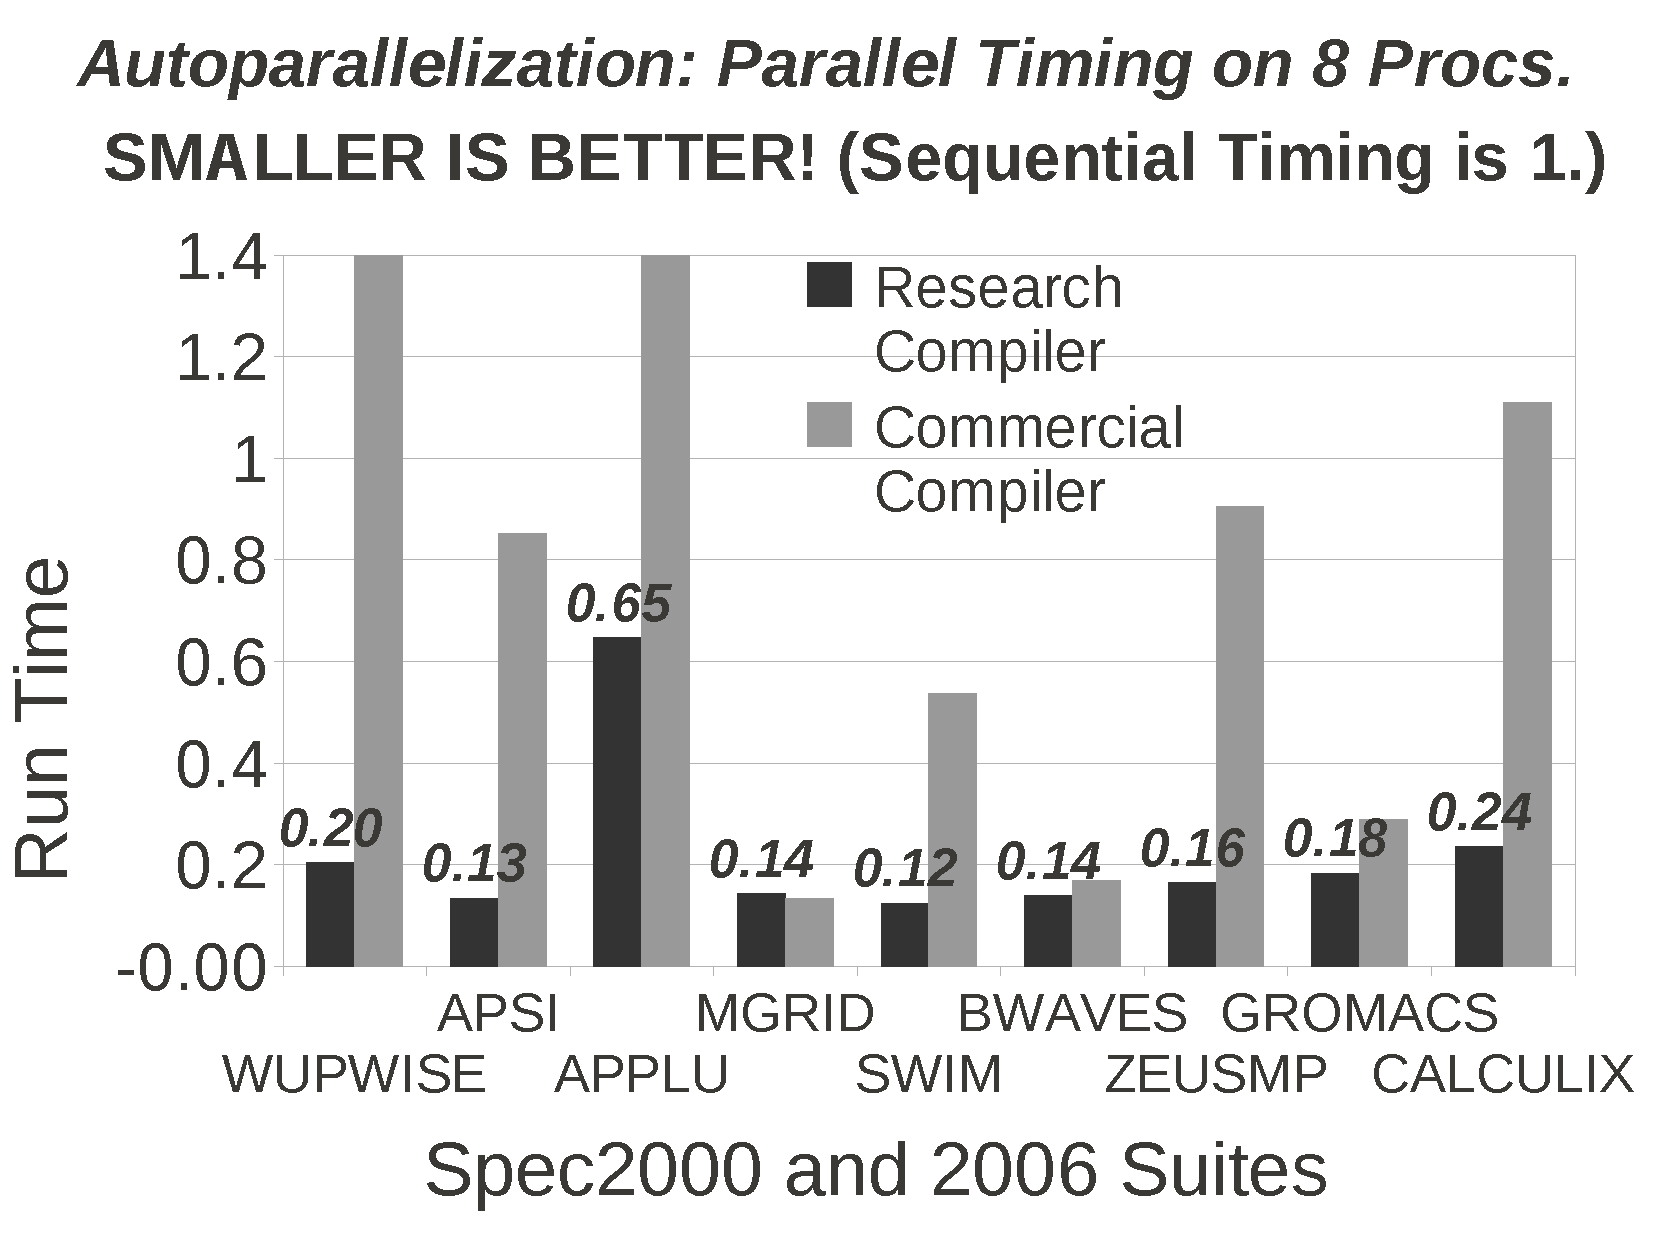
\includegraphics[scale=0.215]{ParTeaserFigs/Spec2006Res}
%\includegraphics<2-4>[scale=0.215]{ParTeaserFigs/PerfectResO2.pdf}


\begin{frame}[fragile,t]
  \frametitle{Impact of Loop Fusion/Distribution}

Speedup on mobile and gaming {\sc gpgpu}s with loop fusion \\ 
\emphb{ON} (blue) and loop distribution \empr{ON} (red). HIGHER is BETTER!
\smallskip
\begin{center} 
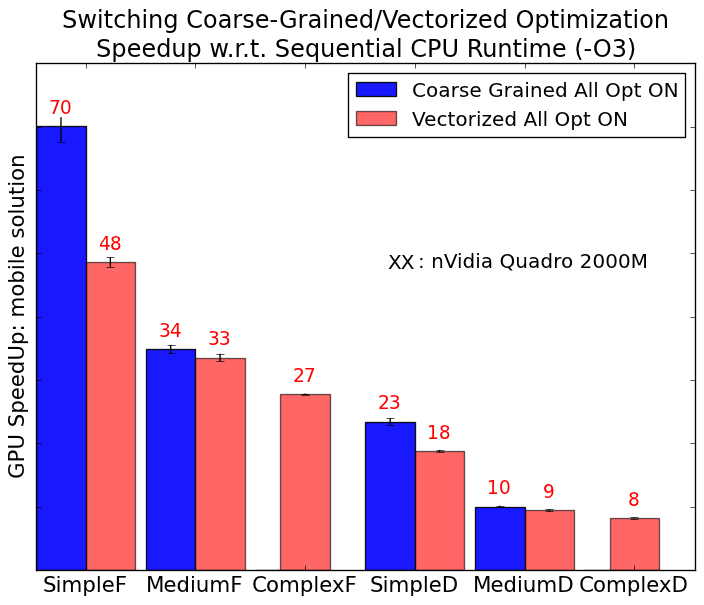
\includegraphics[height=25.5ex]{ParTeaserFigs/optimizations-GPU-CG-1.png} 
$\mbox{ }\mbox{ }\mbox{ }\mbox{ }$
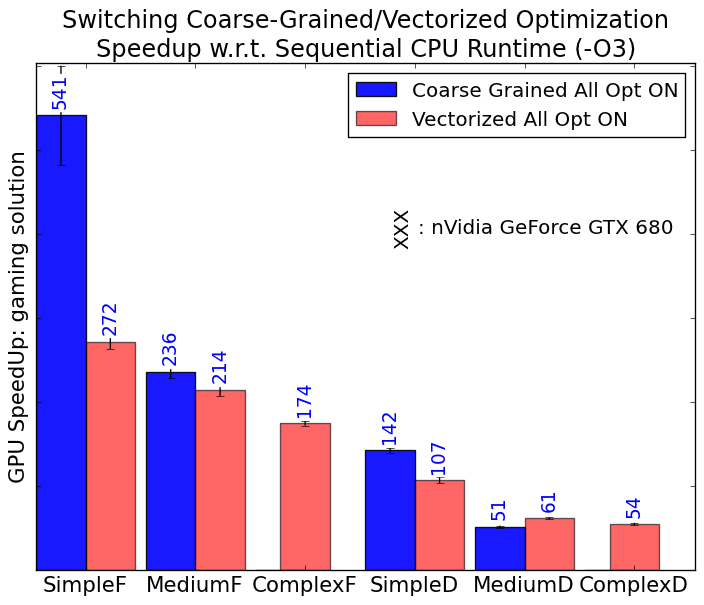
\includegraphics[height=25.5ex]{ParTeaserFigs/optimizations-GPU-CG-0.png} 
\end{center} 
\smallskip

Impact is input-sensitive; but a cost model can chose at runtime the better alternative.

\end{frame}


\begin{frame}[fragile,t]
  \frametitle{Impact of Memory-Coalescing Optimization}

Speedup on mobile and gaming {\sc gpgpu}s with memory-coalescing \\ 
optimization \empr{ON} (red) and \emphb{OFF} (blue). HIGHER is BETTER!
\smallskip
\begin{center} 
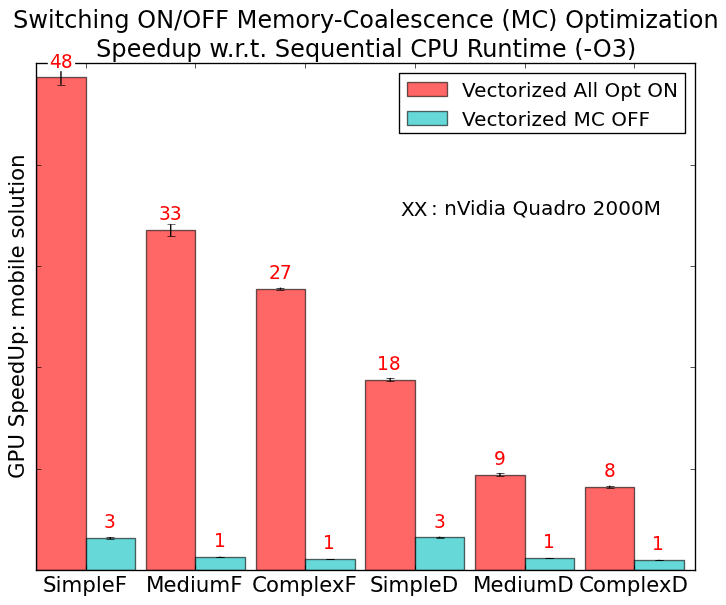
\includegraphics[height=25.5ex]{ParTeaserFigs/optimizations-GPU-MC-1.png} 
$\mbox{ }\mbox{ }\mbox{ }\mbox{ }$
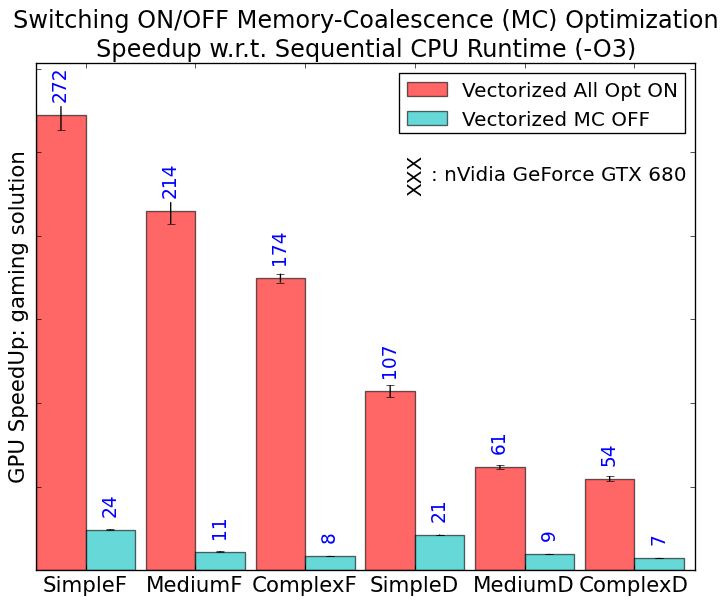
\includegraphics[height=25.5ex]{ParTeaserFigs/optimizations-GPU-MC-0.png} 
\end{center} 
\smallskip

\emp{Not natural but effective transformation, hence suited to be implemented in the repertoire of an optimizing compiler.}

\end{frame}








\section{Imperative Context: Direction-Vector Analysis of Parallelism}

\begin{frame}[fragile]
	\tableofcontents[currentsection]
\end{frame}


\begin{frame}[fragile,t]
  \frametitle{Problem Statement} % of CPU, Multicores, GPGPU

Iterations are ordered {\em lexicographically}, w.r.t. how they 
occur in the sequential execution, e.g., first loop next, 
{\tt(j=1,i=4) < (j=2,i=3)}.

%[fontsize=\small]
\begin{block}{Three Loop Examples}
\begin{colorcode}
DO i = 1, N             DO i = 2, N                 DO i = 2, N
  DO j = 1, N             DO j = 2, N                 DO j = 1, N 
    A[j,i] = A[j,i] ..      A[j,i] = A[j-1,i-1]...        A[i,j] = A[i-1,j+1]...
  ENDDO                     B[j,i] = B[j-1,i]...      ENDDO
ENDDO                   ENDDO ENDDO                 ENDDO
\end{colorcode}
\end{block} 

\bigskip

\begin{itemize}
    \item Which of the three loop nests is amenable to parallelization?\smallskip
    \item Loop interchange is one of the most simple and useful code transformations,
            e.g., used to enhance locality of reference, parallel-loop granularity,
            and even to ``create'' parallelism.\smallskip
    \item In which loop nest is it safe to interchange the loops?
\end{itemize}


\end{frame}


\begin{frame}[fragile,t]
  \frametitle{Loop-Nest Dependencies} % of CPU, Multicores, GPGPU

Iterations are ordered {\em lexicographically}, w.r.t. how they 
occur in the sequential execution, e.g., first loop next, 
{\tt(j=1,i=4) < (j=2,i=3)}.

%[fontsize=\small]
\begin{block}{Three Loop Examples}
\begin{colorcode}
DO i = 1, N             DO i = 2, N                 DO i = 2, N
  DO j = 1, N             DO j = 2, N                 DO j = 1, N 
    A[j,i] = A[j,i] ..      A[j,i] = A[j-1,i-1]...        A[i,j] = A[i-1,j+1]...
  ENDDO                     B[j,i] = B[j-1,i]...      ENDDO
ENDDO                   ENDDO ENDDO                 ENDDO
\end{colorcode}
\end{block} 

\hspace{-3ex}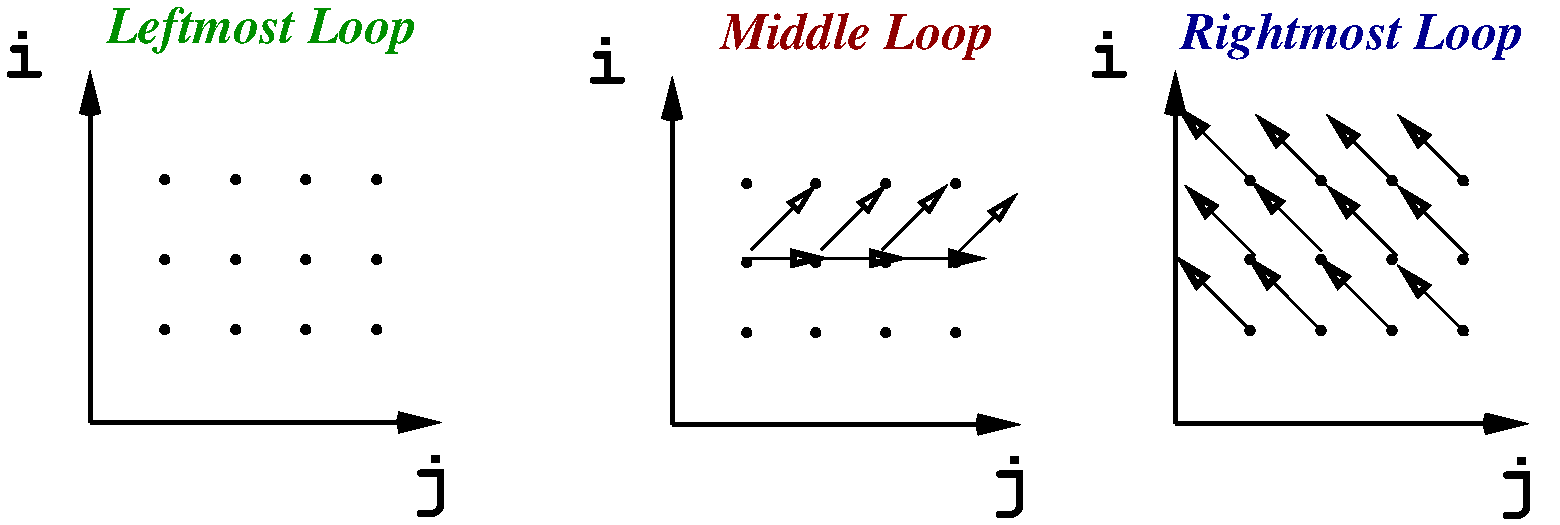
\includegraphics[height=23ex]{ParTeaserFigs/LoopDeps}  

\end{frame}



\begin{frame}[fragile,t]
  \frametitle{Definition of a Dependency} % of CPU, Multicores, GPGPU

\begin{block}{Load-Store Classification of Dependencies}
\begin{colorcode}
True Dependency (RAW)    Anti Dependency (WAR)    Output dependency (WAW)
S1    X  = ..            S1    .. = X             S1    X = ...            
S2    .. = X             S2    X  = ..            S2    X = ...
\end{colorcode}
\end{block} 

\smallskip

{\bf Th. Loop Dependence:} There is a dependence from statement $S1$ to $S2$
in a loop nest {\em iff} $\exists$ iterations $i$, $j$ such that:
\begin{description}
    \item[1.] $i < j$ or $i = j$ and $\exists$ a path from $S1$ to $S2$ such that
    \item[2.] $S1$ accesses memory location $M$ on iteration $i$, and
    \item[3.] $S2$ accesses memory location $M$ on iteration $j$, and
    \item[4.] one of these accesses is a write.
\end{description}

\bigskip

We are most interested in cross iteration dependencies, i.e., $i < j$.\\\smallskip
If $i = j$ the dependency is within the same iteration, i.e., 
does not affect parallelism, since an iteration is executed sequentially.


\end{frame}


\begin{frame}[fragile,t]
  \frametitle{Direction Vectors} % of CPU, Multicores, GPGPU

\begin{block}{Three Loop Examples}
\begin{colorcode}
  DO i = 1, N            DO i = 2, N               DO i = 2, N
    DO j = 1, N            DO j = 2, N               DO j = 1, N 
S1    A[j,i]=A[j,i]..  S1   A[j,i]=A[j-1,i]...   S1    A[i,j]=A[i-1,j+1]...
    ENDDO              S2   B[j,i]=B[j-1,i-1]...     ENDDO
  ENDDO                  ENDDO ENDDO               ENDDO
\end{colorcode}
\end{block} 



\smallskip

Dependencies depicted via an edge {\em from} the stmt that executes first
in the loop nest, i.e., {\em the source}, {\em to} the one that executes later, {\em the sink}.

\smallskip

{\bf Def. Dependence Direction:} Assume $\exists$ a dependence from $S1$ in iteration $q$
to $S2$ in $t$ ($q<t$). \emp{\em Dependence-direction vector $D(q,t)$}:
\begin{description}
    \item[1.] $D(q,t)_k = $~``{\tt{}<}'' if $t_k - q_k > 0$,
    \item[2.] $D(q,t)_k = $~``{\tt{}=}'' if $t_k - q_k = 0$,
    \item[3.] $D(q,t)_k = $~``{\tt{}>}'' if $t_k - q_k < 0$.
\end{description}

\bigskip
\alert{Let's write the direction vectors for the three loop nests.}
\end{frame}


\begin{frame}[fragile,t]
  \frametitle{Parallelism and Loop Interchange} % of CPU, Multicores, GPGPU

\begin{block}{Direction Vectors/Matrix for Three Loops }
\begin{colorcode}
  DO i = 1, N            DO i = 2, N               DO i = 2, N
    DO j = 1, N            DO j = 2, N               DO j = 1, N 
S1    A[j,i]=A[j,i]..  S1   A[j,i]=A[j-1,i]...   S1    A[i,j]=A[i-1,j+1]...
    ENDDO              S2   B[j,i]=B[j-1,i-1]...     ENDDO
  ENDDO                  ENDDO ENDDO               ENDDO

For S1\mymath{\rightarrow}S1: j1 = j2    For S1\mymath{\rightarrow}S1: j1 = j2-1          For S1\mymath{\rightarrow}S1: i1 = i2-1
            i1 = i2                i1 = i2                        j1 = j2+1
(i2,j2)-(i1,j1)=         (i2,j2)-(i1,j1)=\emp{[=,<]}        (i2,j2)-(i1,j1)=\emp{[<,>]}
\emp{[=,=]}                  For S2\mymath{\rightarrow}S2: j1 = j2-1
                                   i1 = i2-1
                         (i2,j2)-(i1,j1)=\emp{[<,<]}
\end{colorcode}
\end{block} 

{\bf Th. Parallelism:} A loop in a loop nest is parallel {\em iff} all its directions
are either {\tt =} or there exists an outer loop whose corresp. direction is {\tt <}. 

\smallskip

{\bf Th. Loop Interchange:} A column permutation of the loops in a loop nest 
is legal {\em iff} permuting the direction matrix in the same way {\em does NOT result}
in a {\tt >} direction as the leftmost non-{\tt{}=} direction in a row. 


\end{frame}


\begin{frame}[fragile,t]
  \frametitle{Parallelism and Loop Interchange} % of CPU, Multicores, GPGPU

\begin{block}{Direction Vectors/Matrix for Three Loops }
\begin{colorcode}
  DO i = 1, N            DO i = 2, N               DO i = 2, N
    DO j = 1, N            DO j = 2, N               DO j = 1, N 
S1    A[j,i]=A[j,i]..  S1   A[j,i]=A[j-1,i]...   S1    A[i,j]=A[i-1,j+1]...
    ENDDO              S2   B[j,i]=B[j-1,i-1]...     ENDDO
  ENDDO                  ENDDO ENDDO               ENDDO

For S1\mymath{\rightarrow}S1: j1 = j2    For S1\mymath{\rightarrow}S1: j1 = j2-1          For S1\mymath{\rightarrow}S1: i1 = i2-1
            i1 = i2                i1 = i2                    j1 = j2+1
(i2,j2)-(i1,j1)=         (i2,j2)-(i1,j1)=\emp{[=,<]}        (i2,j2)-(i1,j1)=\emp{[<,>]}
\emp{[=,=]}                  For S2\mymath{\rightarrow}S2: j1 = j2-1
                                   i1 = i2-1
                         (i2,j2)-(i1,j1)=\emp{[<,<]}
\end{colorcode}
\end{block} 

Interchange is safe for the first and second nests, but not for the third!\\
e.g., \emp{\tt [=,<]}$~~~\rightarrow~~~$ \emph{\tt [<,=]}$~~~~~~~~~$(for the second loop nest)\\
$~~~~~~$\emp{\tt [<,<]}$~~~~~~~~~~~~$\emph{\tt [<,<]}

\smallskip

After interchange, loop $j$ of the second loop nest is parallel.

\bigskip

{\bf Corollary:} A parallel loop can be always interchanged inwards.
\end{frame}


\begin{frame}[fragile,t]
  \frametitle{Dependency Graph and Loop Distribution} % of CPU, Multicores, GPGPU

\begin{block}{Vectorization Example}
\begin{columns}
\column{0.34\textwidth}
\begin{colorcode}[fontsize=\scriptsize]
  DO i = 2, N
\emp{S1  A[i] = B[i-1] ...}
\alert{S2  B[i] = B[i-1] ...}
  ENDDO  

For S2\mymath{\rightarrow}S1: i1 = i2-1, \emp{[<]}
For S2\mymath{\rightarrow}S2: i1 = i2-1, \emp{[<]}
\end{colorcode} 
\column{0.27\textwidth}
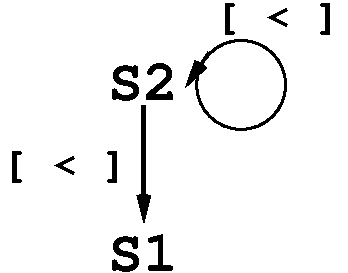
\includegraphics[height=12ex]{ParTeaserFigs/LoopDistr}  
\column{0.30\textwidth}
\begin{colorcode}[fontsize=\scriptsize]
  \alert{DO} i = 2, N
S2  B[i] = B[i-1] ...
  \alert{ENDDO}

  \emphh{DOALL} i = 2, N
\emp{S1  A[i] = B[i-1] ...}
  \emphh{ENDDOALL}
\end{colorcode}
\end{columns}
\end{block}

\smallskip

{\bf Def. Dependency Graph:} edges from the source of the dependency, i.e., early iteration, 
to the sink, i.e., later iteration. 

\smallskip

{\bf Th. Loop Distribution:} Statements that are in a dependence cycle remain in one (sequential) loop.
The others are distributed to separate loops in graph order; if no cycle then parallel loops.

\bigskip

{\bf Corollary:} It is always legal to distribute a parallel loop; potentially you need
array expansion if output dependencies are present.
\end{frame}


\begin{frame}[fragile,t]
  \frametitle{Block Tiling via Loop Distribution and Interchange} % of CPU, Multicores, GPGPU
\vspace{-2ex}
\begin{block}{Matrix Multiplication Example: First Tile all Loops (Always Safe)}
\begin{columns}
\column{0.3\textwidth}\vspace{-2ex}
\begin{colorcode}[fontsize=\scriptsize]
DO i = 1, N   \emphh{// Parallel}
  DO j = 1, N  \emphh{// Parallel}
    C[i,j] = 0.0
    
    DO k = 1, N
      C[i,j] += A[k,j] * B[i,k]
    ENDDO
  ENDDO
ENDDO
\end{colorcode} 
\column{0.05\textwidth}\vspace{-2ex}
\begin{colorcode}[fontsize=\scriptsize]
\emp{LOOP}
\emp{------->}
\emp{TILING}



\end{colorcode}
\column{0.45\textwidth}\vspace{-2ex}
\begin{colorcode}[fontsize=\scriptsize]
DO ii = 1, N, L  
  \emp{DO i = ii, ii+L-1} 
    DO jj = 1, N, L
      \emp{DO j = jj, jj+L-1}  
        C[i,j] = 0.0
        DO kk = 1, N, L
          \emp{DO k = kk, kk+L-1}
            C[i,j] += A[k,j]*B[i,k]
ENDDO ENDDO ENDDO ENDDO ENDDO ENDDO
\end{colorcode}
\end{columns}
\end{block}
\vspace{-2ex}
\begin{block}{Loops {\tt i} and {\tt j} are parallel: Move Inside, Then Distribute}
\begin{columns}
\column{0.3\textwidth}\vspace{-2ex}
\begin{colorcode}[fontsize=\scriptsize]
DO ii = 1, N, L  
  DO jj = 1, N, L
    \emp{DO i = ii, ii+L-1} 
      \emp{DO j = jj, jj+L-1}  
        C[i,j] = 0.0
        DO kk = 1, N, L
          DO k = kk, kk+L-1
            C[i,j] += A[k,j]*B[i,k]
ENDDO ENDDO ENDDO ENDDO ENDDO ENDDO
\end{colorcode} 
\column{0.1\textwidth}\vspace{-2ex}
\begin{colorcode}[fontsize=\scriptsize]
\emp{DISTRIBUTE}
\emp{LOOPS i,j}
\emp{--------->}
\emp{AND MOVE}
\emp{THEM}
\emp{INSIDE kk}




\end{colorcode}
\column{0.45\textwidth}\vspace{-2ex}
\begin{colorcode}[fontsize=\scriptsize]
\emphh{DOALL} ii = 1, N, L  
  \emphh{DOALL} jj = 1, N, L
    \emp{DO i = ii, ii+L-1} 
      \emp{DO j = jj, jj+L-1}  
        C[i,j] = 0.0
    ENDDO ENDDO
    DO kk = 1, N, L
      \emp{DO i = ii, ii+L-1} 
        \emp{DO j = jj, jj+L-1}  
          \emp{DO k = kk, kk+L-1}
            C[i,j] += A[k,j]*B[i,k]
ENDDO ENDDO ENDDO ENDDO ENDDO ENDDO
\end{colorcode}
\end{columns}
\end{block}


\end{frame}


\section{Imperative Context: Summarization of Array Indexes}
\begin{frame}[fragile]
	\tableofcontents[currentsection]
\end{frame}


\begin{frame}[fragile,t]
  \frametitle{Interprocedural Summarization of Array Indexes}


\begin{block}{ Independence-Summary Simple Example } \vspace{-1ex}
\begin{columns} 
\column{0.35\textwidth} 
\begin{colorcode}[fontsize=\scriptsize]
DO i = 1, N
  A(\emp{i+100}) = ...
  IF (x > 0) THEN
    ... = A(\emp{i})
  ENDIF
ENDDO
\end{colorcode}
\column{0.55\textwidth} 
\begin{center} \hspace{-4ex}
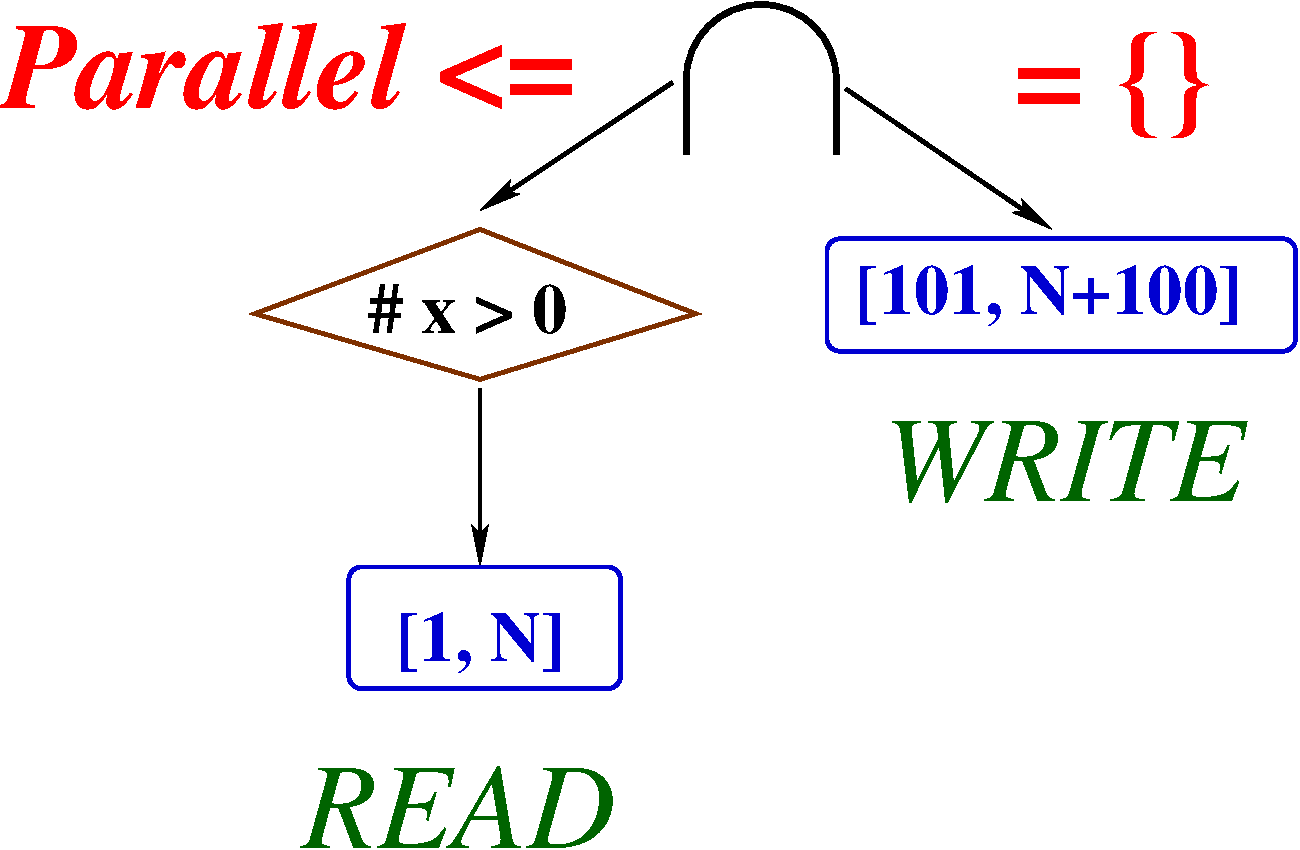
\includegraphics[height=15ex]{ParTeaserFigs/SimpleInd}
\end{center}
\end{columns}
\end{block}


        \begin{itemize}
            \item Techniques that analyze read-write pairs of accesses become
                    very conservative on larger loops with non-trivial control flow.\smallskip   
            \item {\em Alternative:} inter-procedural summarization + model loop independence 
                    via an equation on summaries of shape $S = \emptyset$\\\smallskip 
            \item Decrease overhead by extracting lightweight predicates that prove 
                    independence at runtime, e.g., {\tt x~$\leq$~0~~$\vee$~~N~<~100}.
        \end{itemize} 

\bigskip

\alert{Show Calculix from \textsc{Spec2006}}!

\end{frame}


\begin{frame}[fragile,t]
  \frametitle{Building RO, RW, WF Summaries Interprocedurally}

Summaries ({\sc ro}, {\sc rw}, {\sc wf}) are
\begin{itemize}
    \item constructed via a bottom-up parse of the {\sc call} and {\sc cd} graphs,
    \item structural data-flow equations dictate how to compose consecutive regions,
            aggregate/translate across loops/callsites, ...
\end{itemize}

\pause

\begin{block}{Simplified {\tt solvh\_do20} from {\tt dyfesm}} \vspace{-1ex}
\begin{columns} 
\column{0.45\textwidth}
\begin{colorcode}[fontsize=\scriptsize]
\emp{DO i = 1, N}
    CALL geteu (XE(IA(i)), NP, SYM)
    CALL matmul(XE(IA(i)), NS)
\emp{ENDDO}

SUBROUTINE matmul(XE, NS)
  INTEGER NS, XE(*)
  DO j = 1, NS
    ...   = XE(j) ...
    XE(j) = ...
  ENDDO 
END
\end{colorcode}
\column{0.45\textwidth} 
\begin{colorcode}[fontsize=\scriptsize]
SUBROUTINE geteu(XE, NP, SYM)
  INTEGER NP, SYM, XE(16, *)
  
  IF (SYM .NE. 1) THEN
    DO i = 1, NP
      DO j = 1, 16
        XE(j, i) = ...
      ENDDO 
    ENDDO
  ENDIF
END
\end{colorcode}
\end{columns}
\end{block}

\end{frame}


%%%%%%%%%%%%%%%%%%%%%%%%%%%%%%
%%%%% SUBROUTINE getue
%%%%%%%%%%%%%%%%%%%%%%%%%%%%%%

\begin{frame}[fragile,t]
  \frametitle{Summarizing Subroutine {\tt geteu}}

\begin{block}{WF summary for {\tt geteu}; RO$_{geteu}$ $=$ RW$_{geteu}$ $= \emptyset$ } \vspace{-1ex}
\begin{columns} 
\column{0.45\textwidth} 
\begin{colorcode}[fontsize=\scriptsize]
\mymath{S\myindx{geteu}}  SUBROUTINE geteu(XE, NP, SYM)
         INTEGER NP, SYM, XE(16, *)  
\mymath{S\myindx{IF}}       \emph{IF (SYM .NE. 1) THEN}
\mymath{S\myindx{Li}}         \emp{DO i = 1, NP}
\mymath{S\myindx{Lj}}           \emp{DO j = 1, 16}
\mymath{S\myindx{WF}}             \alert{XE(j, i)} = ...
             \emp{ENDDO} 
           \emp{ENDDO}
         \emph{ENDIF}
       END
\end{colorcode}
\column{0.45\textwidth}
\begin{colorcode}[fontsize=\scriptsize]








\alert{\mymath{WF\myindu{XE}\myindx{S\myindx{WF}} = \{16*i+j-1\}}}
\end{colorcode}
\end{columns}
\end{block}


\begin{itemize}
    \item Loop Aggregation uses (intuitively) interval arithmetic: \smallskip
    \item Loop $i$: $\{16*i + j - 1 \mbox{ }\mbox{ }|\mbox{ } j \in \{1..\mbox{ }16\}\} \rightarrow \emp{16*i + [0,15]}$ \smallskip
    \item Loop $j$: $\{16*i + [0,15] \mbox{ }|\mbox{ } i \in \{1..NP\}\} \rightarrow \emp{[0, 16*NP-1]}$  \smallskip
    \item Branches introduce predicated nodes, e.g., \emph{$WF^{XE}_{S_{if}} = WF^{XE}_{S_{geteu}}$} 
\end{itemize}
\end{frame}

%%%%%%%%%%%%%%%%%%%%%%%%%%%%%%%%%%%%%%%%%%%%%%%%%%%%

\begin{frame}[fragile,t]
  \frametitle{Summarizing Subroutine {\tt geteu}}

\begin{block}{WF summary for {\tt geteu}; RO$_{geteu}$ $=$ RW$_{geteu}$ $= \emptyset$ } \vspace{-1ex}
\begin{columns} 
\column{0.45\textwidth} 
\begin{colorcode}[fontsize=\scriptsize]
\mymath{S\myindx{geteu}}  SUBROUTINE geteu(XE, NP, SYM)
         INTEGER NP, SYM, XE(16, *)  
\mymath{S\myindx{IF}}       \emph{IF (SYM .NE. 1) THEN}
\mymath{S\myindx{Li}}         \emp{DO i = 1, NP}
\mymath{S\myindx{Lj}}           \emp{DO j = 1, 16}
\mymath{S\myindx{WF}}             \alert{XE(j, i)} = ...
             \emp{ENDDO} 
           \emp{ENDDO}
         \emph{ENDIF}
       END
\end{colorcode}
\column{0.45\textwidth}
\begin{colorcode}[fontsize=\scriptsize]

\emp{\mymath{WF\myindu{XE}\myindx{S\myindx{Lj}} = 16*i + [0,15]}}

\alert{\mymath{WF\myindu{XE}\myindx{S\myindx{WF}} = \{16*i+j-1\}}}
\end{colorcode}
\end{columns}
\end{block}


\begin{itemize}
    \item Loop Aggregation uses (intuitively) interval arithmetic: \smallskip
    \item Loop $i$: $\{16*i + j - 1 \mbox{ }\mbox{ }|\mbox{ } j \in \{1..\mbox{ }16\}\} \rightarrow \emp{16*i + [0,15]}$ \smallskip
    \item Loop $j$: $\{16*i + [0,15] \mbox{ }|\mbox{ } i \in \{1..NP\}\} \rightarrow \emp{[0, 16*NP-1]}$  \smallskip
    \item Branches introduce predicated nodes, e.g., \emph{$WF^{XE}_{S_{if}} = WF^{XE}_{S_{geteu}}$} 
\end{itemize}
\end{frame}


%%%%%%%%%%%%%%%%%%%%%%%%%%%%%%%%%%%%%%%%%%%%%%%%%%%%

\begin{frame}[fragile,t]
  \frametitle{Summarizing Subroutine {\tt geteu}}

\begin{block}{WF summary for {\tt geteu}; RO$_{geteu}$ $=$ RW$_{geteu}$ $= \emptyset$ } \vspace{-1ex}
\begin{columns} 
\column{0.45\textwidth} 
\begin{colorcode}[fontsize=\scriptsize]
\mymath{S\myindx{geteu}}  SUBROUTINE geteu(XE, NP, SYM)
         INTEGER NP, SYM, XE(16, *)  
\mymath{S\myindx{IF}}       \emph{IF (SYM .NE. 1) THEN}
\mymath{S\myindx{Li}}         \emp{DO i = 1, NP}
\mymath{S\myindx{Lj}}           \emp{DO j = 1, 16}
\mymath{S\myindx{WF}}             \alert{XE(j, i)} = ...
             \emp{ENDDO} 
           \emp{ENDDO}
         \emph{ENDIF}
       END
\end{colorcode}
\column{0.45\textwidth}
\begin{colorcode}[fontsize=\scriptsize]




\emp{\mymath{WF\myindu{XE}\myindx{S\myindx{Li}} = [0,16*NP-1]}}

\emp{\mymath{WF\myindu{XE}\myindx{S\myindx{Lj}} = 16*i + [0,15]}}

\alert{\mymath{WF\myindu{XE}\myindx{S\myindx{WF}} = \{16*i+j-1\}}}
\end{colorcode}
\end{columns}
\end{block}


\begin{itemize}
    \item Loop Aggregation uses (intuitively) interval arithmetic: \smallskip
    \item Loop $i$: $\{16*i + j - 1 \mbox{ }\mbox{ }|\mbox{ } j \in \{1..\mbox{ }16\}\} \rightarrow \emp{16*i + [0,15]}$ \smallskip
    \item Loop $j$: $\{16*i + [0,15] \mbox{ }|\mbox{ } i \in \{1..NP\}\} \rightarrow \emp{[0, 16*NP-1]}$  \smallskip
    \item Branches introduce predicated nodes, e.g., \emph{$WF^{XE}_{S_{if}} = WF^{XE}_{S_{geteu}}$} 
\end{itemize}
\end{frame}


%%%%%%%%%%%%%%%%%%%%%%%%%%%%%%%%%%%%%%%%%%%%%%%%%%%%

\begin{frame}[fragile,t]
  \frametitle{Summarizing Subroutine {\tt geteu}}

\begin{block}{WF summary for {\tt geteu}; RO$_{geteu}$ $=$ RW$_{geteu}$ $= \emptyset$ } \vspace{-1ex}
\begin{columns} 
\column{0.45\textwidth} 
\begin{colorcode}[fontsize=\scriptsize]
\mymath{S\myindx{geteu}}  SUBROUTINE geteu(XE, NP, SYM)
         INTEGER NP, SYM, XE(16, *)  
\mymath{S\myindx{IF}}       \emph{IF (SYM .NE. 1) THEN}
\mymath{S\myindx{Li}}         \emp{DO i = 1, NP}
\mymath{S\myindx{Lj}}           \emp{DO j = 1, 16}
\mymath{S\myindx{WF}}             \alert{XE(j, i)} = ...
             \emp{ENDDO} 
           \emp{ENDDO}
         \emph{ENDIF}
       END
\end{colorcode}
\column{0.45\textwidth}
\begin{colorcode}[fontsize=\scriptsize]
          \emph{\mymath{(SYM \neq 1)}}
\emph{\mymath{WF\myindu{XE}\myindx{S\myindx{IF}} =}       \mymath{\downarrow}}
          \emph{\mymath{[0,16*NP-1]}}

\emp{\mymath{WF\myindu{XE}\myindx{S\myindx{Li}} = [0,16*NP-1]}}

\emp{\mymath{WF\myindu{XE}\myindx{S\myindx{Lj}} = 16*i + [0,15]}}

\alert{\mymath{WF\myindu{XE}\myindx{S\myindx{WF}} = \{16*i+j-1\}}}
\end{colorcode}
\end{columns}
\end{block}


\begin{itemize}
    \item Loop Aggregation uses (intuitively) interval arithmetic: \smallskip
    \item Loop $i$: $\{16*i + j - 1 \mbox{ }\mbox{ }|\mbox{ } j \in \{1..\mbox{ }16\}\} \rightarrow \emp{16*i + [0,15]}$ \smallskip
    \item Loop $j$: $\{16*i + [0,15] \mbox{ }|\mbox{ } i \in \{1..NP\}\} \rightarrow \emp{[0, 16*NP-1]}$  \smallskip
    \item Branches introduce predicated nodes, e.g., \emph{$WF^{XE}_{S_{if}} = WF^{XE}_{S_{geteu}}$} 
\end{itemize}
\end{frame}


%%%%%%%%%%%%%%%%%%%%%%%%%%%%%%
%%%%% SUBROUTINE getue END
%%%%%%%%%%%%%%%%%%%%%%%%%%%%%%


%%%%% SUBROUTINE MATMULT

\begin{frame}[fragile,t]
  \frametitle{Summarizing Subroutine {\tt matmult}}

\begin{block}{RW summary for {\tt matmul}; RO$_{matmul}$ $=$ WF$_{matmul}$ $= \emptyset$ } \vspace{-1ex}
\begin{columns} 
\column{0.48\textwidth} 
\begin{colorcode}[fontsize=\scriptsize]
\mymath{S\myindx{matmul}}  SUBROUTINE matmul(XE, NS)
          INTEGER NS, XE(*)
\mymath{S\myindx{loop}}       \emph{DO j = 1, NS}
\mymath{S\myindx{RO}}          \alert{...   \hspace{0.5ex}= XE(j) ...}
\mymath{S\myindx{WF}}          \alert{XE(j) = ...}
          \emph{ENDDO}
        END
\end{colorcode}
\column{0.48\textwidth}
\begin{colorcode}[fontsize=\scriptsize]




\alert{\mymath{RO\myindu{XE}\myindx{S\myindx{RO}} = \{j-1\}}}
\alert{\mymath{WF\myindu{XE}\myindx{S\myindx{WF}} = \{j-1\}}}
\end{colorcode}
\end{columns}
\end{block}

\bigskip

\begin{itemize}
    \item Composing read-only $RO_{S_1}$ and write-first $WF_{S_2}$ regions:  \smallskip
    \item $RO = RO_{S_1} - WF_{S_2}$, $WF = WF_{S_2} - RO_{S_1}$, $RW = RO_{S_1} \cap WF_{S_2}$  \smallskip
    \item In our case $RO = \emptyset$, $WF = \emptyset$, \emp{$RW = \{j-1\}$}  \smallskip
    \item Over loop {\tt DO j}:  $RO_{loop} = \emptyset$, $WF_{loop} = \emptyset$, \emph{$RW_{loop} = [0, NS-1]$}  \smallskip
\end{itemize}
\end{frame}

%%%%%%%%%%%%%%%%%%%%%%%%%%%%%%%%%%%%%%%%%%%%%%%%%%%%

%%%%%%%%%%%%%%%%%%%%%%%%%%%%%%%%%%%%%%%%%%%%%%%%%%%%

\begin{frame}[fragile,t]
  \frametitle{Summarizing Subroutine {\tt matmult}}

\begin{block}{RW summary for {\tt matmul}; RO$_{matmul}$ $=$ WF$_{matmul}$ $= \emptyset$ } \vspace{-1ex}
\begin{columns} 
\column{0.48\textwidth} 
\begin{colorcode}[fontsize=\scriptsize]
\mymath{S\myindx{matmul}}  SUBROUTINE matmul(XE, NS)
          INTEGER NS, XE(*)
\mymath{S\myindx{loop}}       \emph{DO j = 1, NS}
\mymath{S\myindx{RO}}          \alert{...   \hspace{0.5ex}= XE(j) ...}
\mymath{S\myindx{WF}}          \alert{XE(j) = ...}
          \emph{ENDDO}
        END
\end{colorcode}
\column{0.48\textwidth}
\begin{colorcode}[fontsize=\scriptsize]


\emp{\mymath{S\myindx{RO} \diamond S\myindx{WF} = \{\emptyset, \emptyset, RW=\{j-1\}\}}}

\alert{\mymath{RO\myindu{XE}\myindx{S\myindx{RO}} = \{j-1\}}}
\alert{\mymath{WF\myindu{XE}\myindx{S\myindx{WF}} = \{j-1\}}}
\end{colorcode}
\end{columns}
\end{block}

\bigskip

\begin{itemize}
    \item Composing read-only $RO_{S_1}$ and write-first $WF_{S_2}$ regions:  \smallskip
    \item $RO = RO_{S_1} - WF_{S_2}$, $WF = WF_{S_2} - RO_{S_1}$, $RW = RO_{S_1} \cap WF_{S_2}$  \smallskip
    \item In our case $RO = \emptyset$, $WF = \emptyset$, \emp{$RW = \{j-1\}$}  \smallskip
    \item Over loop {\tt DO j}:  $RO_{loop} = \emptyset$, $WF_{loop} = \emptyset$, \emph{$RW_{loop} = [0, NS-1]$}  \smallskip
\end{itemize}
\end{frame}


\begin{frame}[fragile,t]
  \frametitle{Summarizing Subroutine {\tt matmult}}

\begin{block}{RW summary for {\tt matmul}; RO$_{matmul}$ $=$ WF$_{matmul}$ $= \emptyset$ } \vspace{-1ex}
\begin{columns} 
\column{0.48\textwidth} 
\begin{colorcode}[fontsize=\scriptsize]
\mymath{S\myindx{matmul}}  SUBROUTINE matmul(XE, NS)
          INTEGER NS, XE(*)
\mymath{S\myindx{loop}}       \emph{DO j = 1, NS}
\mymath{S\myindx{RO}}          \alert{...   \hspace{0.5ex}= XE(j) ...}
\mymath{S\myindx{WF}}          \alert{XE(j) = ...}
          \emph{ENDDO}
        END
\end{colorcode}
\column{0.48\textwidth}
\begin{colorcode}[fontsize=\scriptsize]
\emph{\mymath{RW\myindu{XE}\myindx{S\myindx{loop}} = [0,NS-1]}}

\emp{\mymath{S\myindx{RO} \diamond S\myindx{WF} = \{\emptyset, \emptyset, RW=\{j-1\}\}}}

\alert{\mymath{RO\myindu{XE}\myindx{S\myindx{RO}} = \{j-1\}}}
\alert{\mymath{WF\myindu{XE}\myindx{S\myindx{WF}} = \{j-1\}}}
\end{colorcode}
\end{columns}
\end{block}

\bigskip

\begin{itemize}
    \item Composing read-only $RO_{S_1}$ and write-first $WF_{S_2}$ regions:  \smallskip
    \item $RO = RO_{S_1} - WF_{S_2}$, $WF = WF_{S_2} - RO_{S_1}$, $RW = RO_{S_1} \cap WF_{S_2}$  \smallskip
    \item In our case $RO = \emptyset$, $WF = \emptyset$, \emp{$RW = \{j-1\}$}  \smallskip
    \item Over loop {\tt DO j}:  $RO_{loop} = \emptyset$, $WF_{loop} = \emptyset$, \emph{$RW_{loop} = [0, NS-1]$}  \smallskip
\end{itemize}
\end{frame}



%%%%% SUBROUTINE MATMULT

\begin{frame}[fragile,t]
  \frametitle{Summarizing Accesses for the Target Loop}

\begin{block}{RW summary for loop {\tt DO i}: RW$^i$ = ? } \vspace{-1ex}
\begin{columns} 
\column{0.48\textwidth} 
\begin{colorcode}[fontsize=\scriptsize]
        INTEGER NS, NP, IA(*), XE(*)
\mymath{S\myindx{loop}}    \emph{DO i = 1, N}
\mymath{S\myindx{WF}}      CALL geteu (XE(IA(i)),NP,SYM)
\mymath{S\myindx{RW}}      CALL matmul(XE(IA(i)),NS)
        \emph{ENDDO}

\emp{\mymath{S\myindx{WF} \diamond S\myindx{RW} = \{\emptyset, WF\myindu{i}=WF\myindx{geteu}, RW\myindu{i}\}}}
\end{colorcode}
\column{0.48\textwidth}
\begin{center}
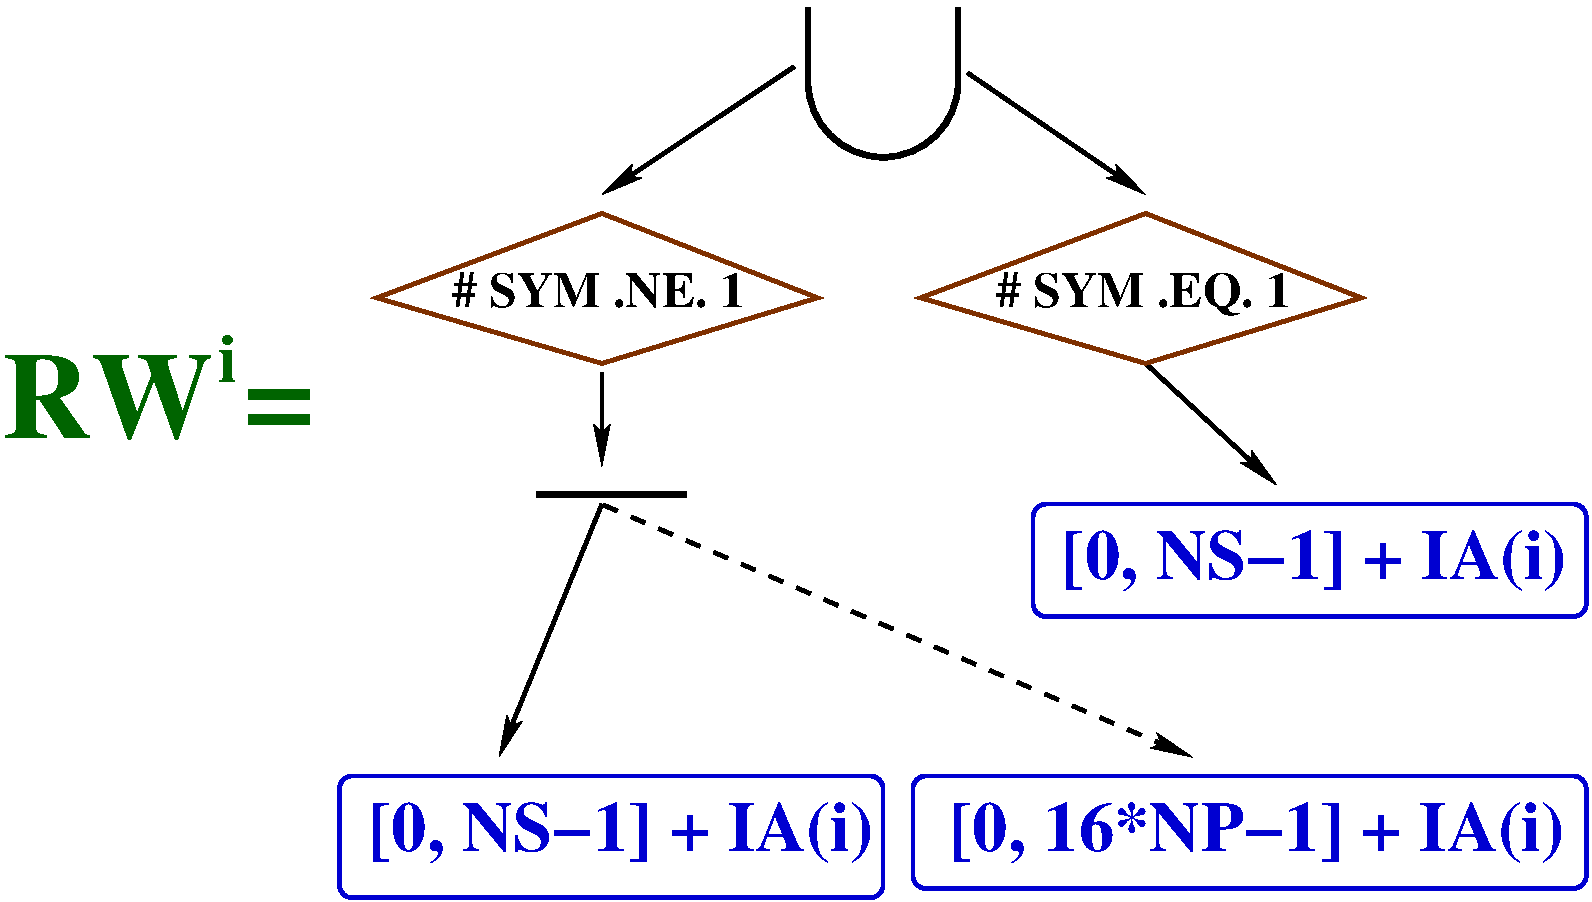
\includegraphics[height=15ex]{ParTeaserFigs/RW_IND_XE}
\end{center}
\end{columns}
\end{block}

\bigskip

In our case, a sufficient condition for {\tt XE} independence is: \bigskip \\ 
$\cup_{i=1}^{N}(RW_i \mbox{ }\cap\mbox{ } (\cup_{k=1}^{i-1}RW_k)) = \emptyset~~~\Leftrightarrow~~~RW_i = \emptyset~~~\Leftrightarrow$

\bigskip

$~~~~~~~~~~~~~~~~~\Leftrightarrow~~~$  
\emph{${\tt SYM}\neq 1\mbox{ }\wedge {\tt NS}\leq 16*{\tt NP}$} 
\end{frame}


\begin{frame}[fragile,t]
  \frametitle{Summary-Based Independence Equations}
\bigskip
Flow and Anti Independence Equation for loop of index \emph{i}:
\begin{equation} \label{FIEq} 
\begin{array}{l r}
S_{find} = \{(\cup_{i=1}^{N} WF_i) \mbox{ }\cap\mbox{ } (\cup_{i=1}^{N} RO_i)\} \mbox{ }\cup & \vspace{1ex} \\ \mbox{ }\mbox{ }\mbox{ }\mbox{ }\mbox{ }\mbox{ }\mbox{ }\mbox{ }\mbox{ }\mbox{ }
\{(\cup_{i=1}^{N} WF_i) \mbox{ }\cap\mbox{ } (\cup_{i=1}^{N} RW_i)\} \mbox{ }\cup & \vspace{1ex} \\ \mbox{ }\mbox{ }\mbox{ }\mbox{ }\mbox{ }\mbox{ }\mbox{ }\mbox{ }\mbox{ }\mbox{ }
\{(\cup_{i=1}^{N}RO_i) \mbox{ }\cap\mbox{ } (\cup_{i=1}^{N}RW_i)\} \mbox{ }\cup  & \vspace{1ex} \\ \mbox{ }\mbox{ }\mbox{ }\mbox{ }\mbox{ }\mbox{ }\mbox{ }\mbox{ }\mbox{ }\mbox{ }
\{ \cup_{i=1}^{N}(RW_i \mbox{ }\cap\mbox{ } (\cup_{k=1}^{i-1}RW_k))\} \mbox{ }\mbox{ }\mbox{ } = \emptyset
\end{array}
\end{equation}

\bigskip

Output Independence Equation for loop of index \emph{i}:
\begin{equation} \label{OIEq} 
\begin{array}{l r}
S_{oind} = \{ \cup_{i=1}^{N}(WF_i \mbox{ }\cap\mbox{ } (\cup_{k=1}^{i-1}WF_k))\} \mbox{ }\mbox{ }\mbox{ } = \emptyset
\end{array}
\end{equation}

\bigskip

Computing $S_{find}$ and $S_{oind}$ solves a more difficult problem than we need, 
i.e., computes the indexes involved in cross-iteration deps. \bigskip

\emp{{\em Loop Independence: when are $S_{find}$ and $S_{oind}$ are empty?}}

\end{frame}


\begin{frame}[fragile,t]
  \frametitle{Key Idea: Predicate-Centric Approach}

\smallskip

{\em Approach centered on extracting arbitrarily-shaped predicates.} 

\bigskip

\begin{block}{Key Idea} 
\begin{columns} 
\column{0.69\textwidth} \vspace{-2ex}
\begin{itemize}
    \item \emp{{\em Source of inaccuracy:}} summary representation not closed under composition w.r.t. set operations. \bigskip
    \item \emph{{\em Language}} representation for summaries ... precise but \emp{expensive} to compute at runtime \bigskip
    \item ``Let's \emph{{\em reason}} about it!'' $\emph{8*NP < NS + 6} \Rightarrow \emp{A - B} = \emptyset \Rightarrow S=\emptyset$!
\end{itemize}
\column{0.33\textwidth} 
\hspace{-2ex}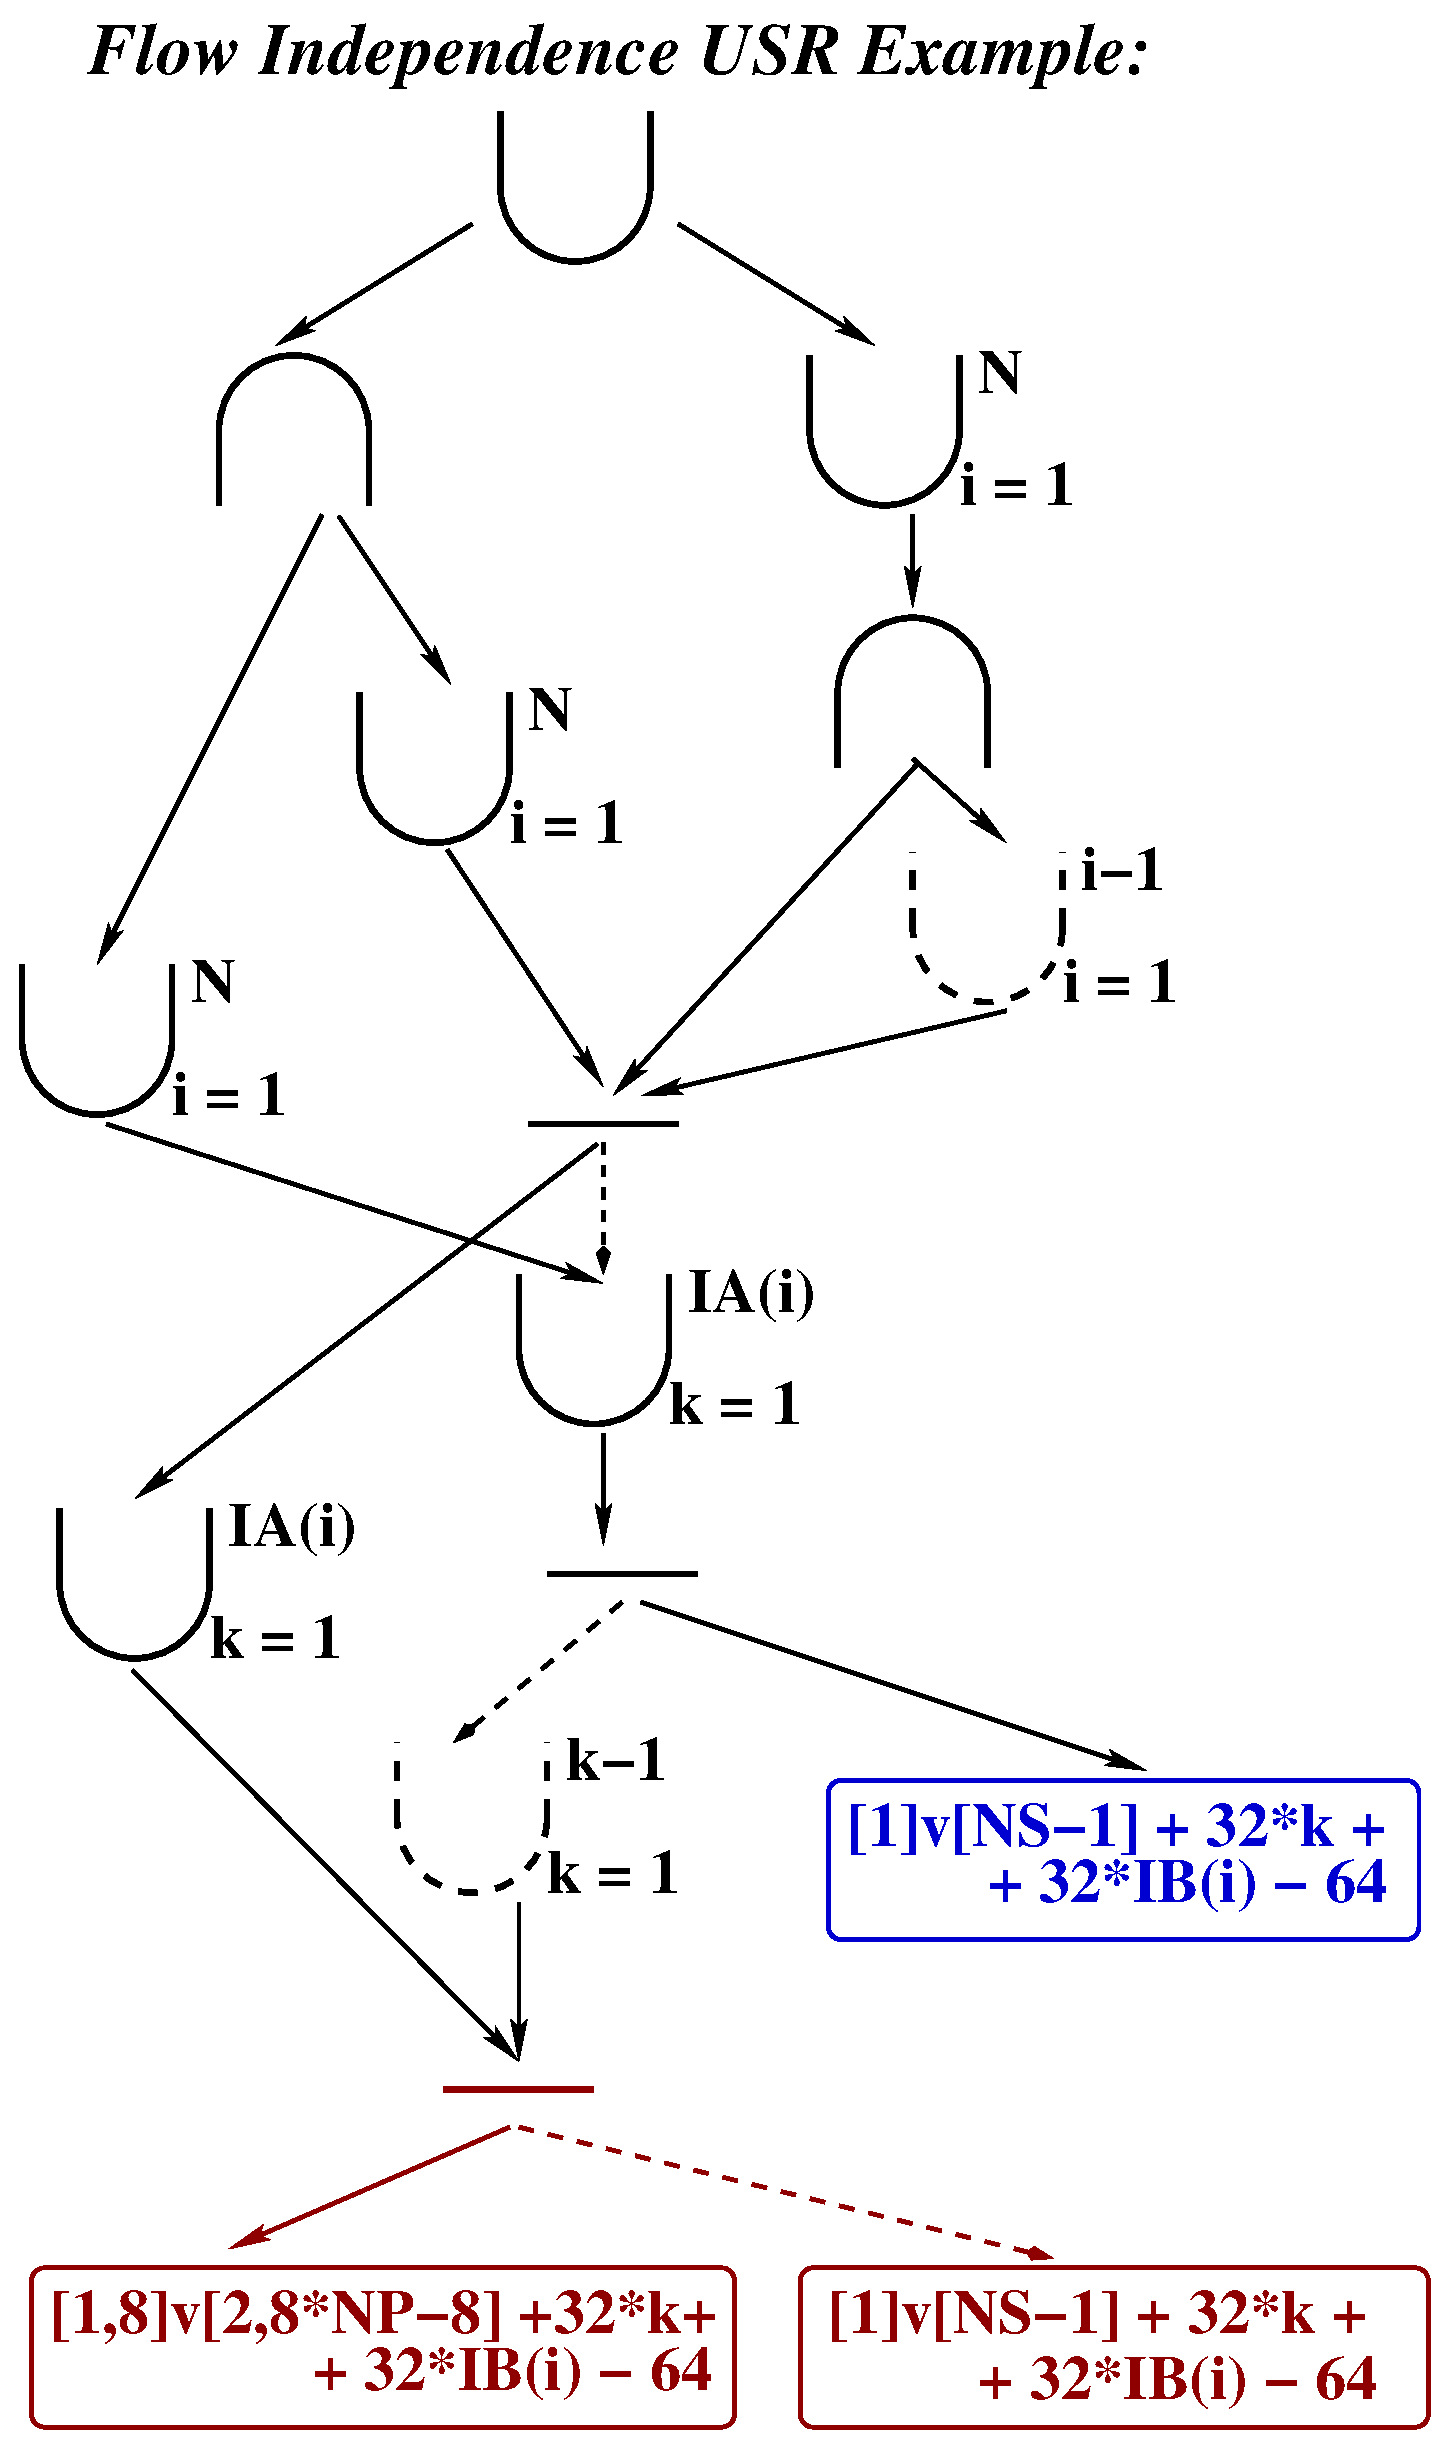
\includegraphics[height=30ex]{ParTeaserFigs/USR_HE_FIND_SOLVH}
\end{columns}
\end{block}

\alert{Show Calculix from \textsc{Spec2006}}!

\end{frame}



\section{Functional Context: List Homomorphisms and Map-Reduce Style}
\begin{frame}[fragile]
	\tableofcontents[currentsection]
\end{frame}

\begin{frame}
  \frametitle{Bird-Meertens Formalism (BMF)} 

BMF: small collection of (i) second-order functions on lists,
    (ii) algebraic identities and theorems, 
    and (iii) a concise notation. 

\begin{block}{BMF Notation:}
\begin{columns} 
\column{0.1\textwidth}\vspace{-4ex}
$\mbox{ }$ \\
$\mbox{ }$ \\
${\tt id}$ \\ 
${\tt .}$\\
$ \oplus, \otimes, \odot$ \\
$ {\tt zipWith} \mbox{ } \odot$\\
$\mbox{ }$\\
$ {\tt map} \mbox{ } f$\\
$\mbox{ }$\\
$ {\tt red} \mbox{ } \odot$\\ %\mbox{ }e_{\odot}$
$\mbox{ }$\\
$\mbox{ }$\\
%$\mbox{ }$\\
%$ {\tt scan}\mbox{ }\odot$\\ %\mbox{ }e_{\odot}
%$\mbox{ }$ \\
%$\mbox{ }$
\column{0.8\textwidth}
identity function, i.e., ${\tt id} : T \rightarrow T, {\tt id}\mbox{ }x = x$ \\
backward functional composition: $(f\mbox{ }.\mbox{ }g)\mbox{ }x = f\mbox{ }(g\mbox{ }x)$ \\
binary associative operators, $\odot :: T \rightarrow T \rightarrow T$ \\
application of $\odot$ to a pair of equal-length lists: \\
${\tt zipWith}\mbox{ }\odot\mbox{ }[x_1,..,x_n]\mbox{ }[y_1,..,y_n]\mbox{ }=\mbox{ }[x_1\odot y_1,..,x_n\odot y_n]$. \\
$f :: T_{1} \rightarrow T_{2}$, ${\tt map} :: [T_{1}] \rightarrow [T_{2}]$, \\
${\tt map} \mbox{ }f\mbox{ } [x_{1},..,x_{n}] \mbox{ }=\mbox{ }[(f\mbox{ }x_{1}),..,(f\mbox{ }x_{n})]$ \\
reduce with binary associative operator $\odot$, ${\tt red}::(T \rightarrow T \rightarrow T) \rightarrow T \rightarrow [T] \rightarrow T$\\
$red~\odot~e_\odot~[x_1,...,x_n]~~=~~e_\odot~\odot~x_1~\odot~...~\odot~x_n$\\ 
%$e_{\odot} = red\mbox{ }\odot\mbox{ }[]$ \\
%${\tt red} \odot [a] = a$, ${\tt red} \odot (x {\tt ++} y) = (red \odot x) \odot (red \odot y)$ \\
%prefix sum: ${\tt scan}::(T \rightarrow T \rightarrow T) \rightarrow T \rightarrow [T] \rightarrow [T] $, \\ ${\tt scan} \odot [x_1,..,x_n] = [x_1, x_1\odot x_2,..,x_1\odot x_2\odot .. \odot x_n]$ 
\end{columns}
\end{block}
\end{frame}


\begin{frame}
  \frametitle{Reducing in Parallel}

\begin{center} 
        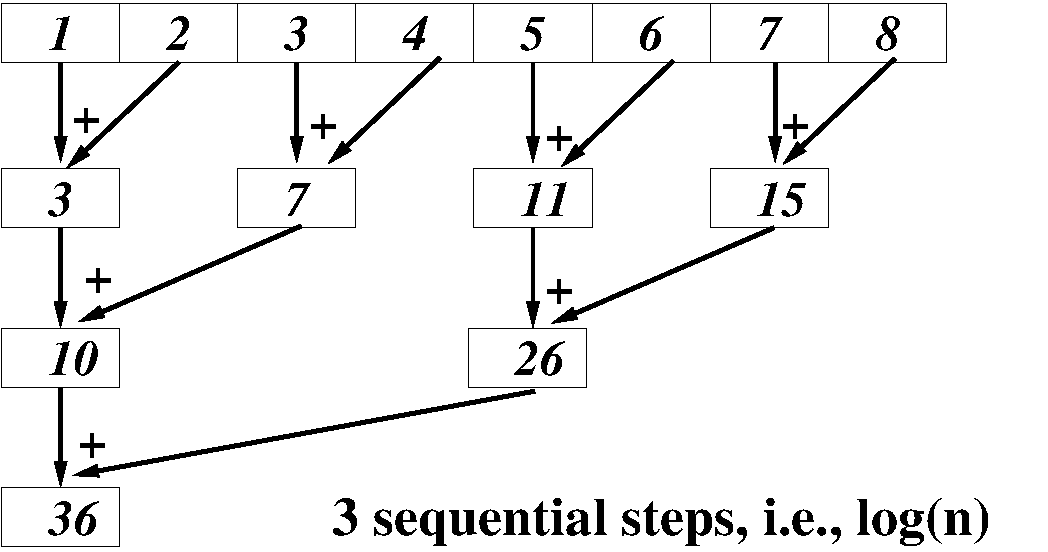
\includegraphics[height=28ex]{ParTeaserFigs/ReduceEg.pdf} 
\end{center} 

We build programs by combining \alert{map} and \alert{reduce}. For example, \smallskip

\emp{scan} (+) [1, 2, 3, 4] $\rightarrow$ [1, 1+2, 1+2+3, 1+2+3+4] $\rightarrow$ [1, 3, 6, 10]\smallskip

can be efficiently implemented as a map reduce.

\end{frame}


\begin{frame}[fragile,t]
  \frametitle{List-Homomorphism and Map-Reduce Equivalence}

Those functions that promote through list concatenation ({\tt ++}):
%$h\mbox{ }(x {\tt ++} y) = (h\mbox{ }x) \odot (h\mbox{ }y)$. More precise:

\begin{mydef}[List Homomorphism]\label{LHomDef}
$h :: [T_1] \rightarrow T_2$ over finite lists is a {\em list homomorphism}
if there exists an associative binary operator $\odot :: T_2 \rightarrow T_2 \rightarrow T_2$,
such that: \\
$\mbox{ }\mbox{ }\mbox{ }\mbox{ }\mbox{ }\mbox{ }\mbox{ }\mbox{ }\mbox{ }$
\emp{$h \mbox{ } (x{\tt ++}y) = (h\mbox{ }x)\mbox{ }\odot\mbox{ }(h\mbox{ }y)$} \\
We denote $h = hom \mbox{ }(\odot) \mbox{ }f\mbox{ }e_{\odot}$, where $f\mbox{ }x = h\mbox{ }[x]$ and $e_{\odot} = h\mbox{ }[]$. 
\end{mydef}


\begin{mytheo}[1st List Homomorphism Theorem (LHTh1)]\label{LHomLema}
Any list homomorphism can be written as the composition
of a reduction and a map:
\emp{$h = hom \mbox{ }(\odot)\mbox{ }f\mbox{ }e_{\odot}\mbox{ }=\mbox{ }(red~(\odot)~e_{\odot})~.~(map~f)$}\\
Conversely, each such composition is a homomorphism.
\end{mytheo}

\bigskip

Theorem tells how to parallelize LHs based on {\tt map-reduce} skeletons.


\end{frame}





\begin{frame}[fragile,t]
  \frametitle{List Homomorphisms (LH)}

\begin{block}{Examples of List Homomorphisms as Map-Reduce} \vspace{-1.5 ex}
\begin{columns}
\column{0.45\textwidth}
\begin{colorcode}[fontsize=\scriptsize]
\emph{len} :: [T] -> Integer
\emph{len} []     = \emp{0}
\emph{len} [x]    = \emp{1}
\emph{len} (x++y) = (\emph{len} x) \emp{+} (\emph{len} y)
\emp{len \mymath{\equiv} (red (+) 0) . (map (fn x \mymath{\Rightarrow} 1))}
-- logical and \emp{\mymath{\wedge}} :: T -> T -> Bool 
-- all elems satisfy p :: T \mymath{\rightarrow} Bool ?
\emph{all\mymath{\myindx{p}}} :: [T] -> Bool
\emph{all\mymath{\myindx{p}}} []     = \emp{True}
\emph{all\mymath{\myindx{p}}} [x]    = \emp{p x} 
\emph{all\mymath{\myindx{p}}} (x++y) = (\emph{all\mymath{\myindx{p}}} x) \emp{\mymath{\wedge}} (\emph{all\mymath{\myindx{p}}} y)
\emp{all\mymath{\myindx{p}} \mymath{\equiv} (red (\emp{\mymath{\wedge}}) True) .} 
        \emp{(map (fn x \mymath{\Rightarrow} p x))}
\mymath{\uparrow} :: Integer -> Integer -> Integer
x \mymath{\uparrow} y = if (x > y) then x else y 
\emph{maxList} :: [Integer] -> Integer
\emph{maxList} []     = \emp{\mymath{-\infty}}
\emph{maxList} [x]    = \emp{x}
\emph{maxList} (x++y) = (\emph{maxList} x) \emp{\mymath{\uparrow}} 
                 (\emph{maxList} y)
\emp{maxList \mymath{\equiv} (red (\mymath{\uparrow}) \mymath{-\infty}) . (map id)}
\end{colorcode}
\column{0.45\textwidth}
\begin{colorcode}[fontsize=\scriptsize]
-- merges two sorted lists
-- into a sorted list
merge :: [T] -> [T] -> [T]
merge :: Ord a => [a] -> [a] -> [a]
merge [] y  = y
merge x  [] = x
merge (x::xs) (y::ys) = 
  if ( x <= y ) 
  then x :: merge xs (y::ys)
  else y :: merge (x::xs) ys 

-- [.] x = [x]  
\emph{mSort} :: [T] -> T
\emph{mSort} []     = \emp{[]}
\emph{mSort} [x]    = \emp{[x]}
\emph{mSort} (x++y) = \emp{merge} (\emph{mSort} x)  
                     (\emph{mSort} y)

\emp{mSort \mymath{\equiv} (red merge []) . (map [.])}
\end{colorcode}
\end{columns}
\end{block}

\end{frame}



\begin{frame}[fragile,t]
  \frametitle{List Homomorphism Invariants}

\begin{mytheo}[Map Fusion/Distribution]\label{Fusion}\vspace{-2ex}
Given unary functions $f$ and $g$ then: \\
$\mbox{ }\mbox{ }\mbox{ }\mbox{ }\mbox{ }\mbox{ }\mbox{ }\mbox{ }$
$({\tt map}~f)~.~({\tt map}~g) \mbox{ }\mbox{ }\equiv\mbox{ }\mbox{ }{\tt map}~(f~{\tt{}.}~g)$ \\
\end{mytheo}


\begin{mytheo}[List-Homomorphism Promotions]\label{LHomInv}\vspace{-2ex}
Given unary function $f$ and an associative binary operator $\odot$ then: \\
$\mbox{ }\mbox{ }\mbox{ }\mbox{ }\mbox{ }\mbox{ }\mbox{ }\mbox{ }$
$({\tt map} \mbox{ }f)\mbox{ }.\mbox{ }({\tt red}\mbox{ }({\tt ++})) \mbox{ }\mbox{ }\equiv\mbox{ }\mbox{ }({\tt red}\mbox{ }({\tt ++}))\mbox{ }.\mbox{ }({\tt map}\mbox{ }({\tt map}\mbox{ }f) )$ \\
$\mbox{ }$ \\
$\mbox{ }\mbox{ }\mbox{ }\mbox{ }\mbox{ }\mbox{ }\mbox{ }\mbox{ }$
$({\tt red}\mbox{ }\odot)\mbox{ }.\mbox{ }({\tt red}\mbox{ }(++)) \mbox{ }\equiv\mbox{ }\mbox{ }({\tt red}\mbox{ }\odot)\mbox{ }.\mbox{ }({\tt map}\mbox{ }({\tt red}\mbox{ }\odot) )$
\end{mytheo}

\bigskip
{\tt (red $\odot$ $e_\odot$) . (map f) $\equiv$ \\
(red~$\odot$~$e_\odot$)~.~(map ((red $\odot$ $e_\odot$)~.~(map f)))~.~distr$_p$},

\smallskip
where {\tt distr$_p$~::~[$\alpha$]~$\rightarrow$~[[$\alpha$]]$_p$, (red~(++)~[])~.~distr$_p$~=~id}. 

\end{frame}


\begin{frame}[fragile,t]
  \frametitle{Exercises}

\alert{Exercise 1}: Function \\
h :: Integral a $=>$ [[a]] $\rightarrow$ a \\
h []   = 0 \\
h (x:xs) = (foldr (+) 0 x) + (h xs) \\
\smallskip
a) Write a list homomorphic implementation of $h$, name it $hh$. \\ \smallskip
b) Write $hh$ in map-reduce style, name it $hMR$ \\ \smallskip
c) Apply the second LH promotion ($\leftarrow$ direction) theorem to optimize it (for example for load-balancing) \\ \smallskip
d) Use the second LH promotion theorem ($\rightarrow$ direction) to chunk the flattened list into $p$ lists, 
    of roughly same number of elements, and to map the computation on each list on one of the $p$ processors; 
    and to finally reduce at the end.  \emph{HINT:} use (distr p) :: [a] $\rightarrow$ [[a]]$_p$ to create a list containing $p$ lists, and invariant {\tt(red (++)[]).(distr p)=id}.  \\ \smallskip
e) Test all versions in Haskell! 
   %To distribute the flattened list into $p$ lists one may use function: \\

%\bigskip

%distr :: Int $\rightarrow$ [a] $\rightarrow$ [[a]] \\
%distr p [] = [] \\
%distr p x = let n = length x in (take n x) : (distr p (drop p x)) \\


\end{frame}


\begin{frame}[fragile,t]
  \frametitle{Conclusion}

\begin{itemize}
    \item Imperative language: low-level, ``heroic effort'', but effective solutions.
            Compiler reverse-engineers users sequential optimizations (hard).\bigskip
    \item Functional language: parallelism via inherently parallel array combinators, 
            that expose a rich algebra at a higher-level of abstraction.\bigskip
    \item Combine the advantages: model the transformations that have proven most useful
            in the imperative context in a simpler way by using the rich algebra of functional constructs.
\end{itemize}

\end{frame}



\end{document}

